\documentclass[conference,final]{IEEEtran}

\usepackage{latex8}
\usepackage[utf8]{inputenc}
\usepackage{url}
\usepackage{float}
\usepackage{times}    
\usepackage{listings}   
\usepackage{paralist}    
\usepackage{wrapfig}    
\usepackage[small,it]{caption}
\usepackage{multirow}
\usepackage{ifpdf}
%\usepackage{srcltx}
\usepackage{subfigure}
\usepackage{xspace}
\usepackage{keyval}  
\usepackage{color}

\definecolor{listinggray}{gray}{0.95}
\definecolor{darkgray}{gray}{0.7}
\definecolor{commentgreen}{rgb}{0, 0.4, 0}
\definecolor{darkblue}{rgb}{0, 0, 0.4}
\definecolor{middleblue}{rgb}{0, 0, 0.7}
\definecolor{darkred}{rgb}{0.4, 0, 0}
\definecolor{brown}{rgb}{0.5, 0.5, 0}

\usepackage[normalem]{ulem}
\makeatletter
\def\cyanuwave{\bgroup \markoverwith{\lower3.5\p@\hbox{\sixly \textcolor{cyan}{\char58}}}\ULon}
\def\reduwave{\bgroup \markoverwith{\lower3.5\p@\hbox{\sixly \textcolor{red}{\char58}}}\ULon}
\def\blueuwave{\bgroup \markoverwith{\lower3.5\p@\hbox{\sixly \textcolor{blue}{\char58}}}\ULon}
\font\sixly=lasy6 % does not re-load if already loaded, so no memory problem.
\makeatother

\newif\ifdraft
\drafttrue

\ifdraft
\newcommand{\onote}[1]{ {\textcolor{cyan} { (***Ole: #1) }}}
\newcommand{\terminology}[1]{ {\textcolor{red} {(Terminology used: \textbf{#1}) }}}
\newcommand{\owave}[1]{ {\cyanuwave{#1}}}
\newcommand{\jwave}[1]{ {\reduwave{#1}}}
\newcommand{\alwave}[1]{ {\blueuwave{#1}}}
\newcommand{\jhanote}[1]{ {\textcolor{red} { ***shantenu: #1 }}}
\newcommand{\alnote}[1]{ {\textcolor{blue} { ***andreL: #1 }}}
\newcommand{\amnote}[1]{ {\textcolor{blue} { ***andreM: #1 }}}
\newcommand{\smnote}[1]{ {\textcolor{brown} { ***sharath: #1 }}}
\newcommand{\msnote}[1]{ {\textcolor{cyan} { ***mark: #1 }}}
\newcommand{\note}[1]{ {\textcolor{magenta} { ***Note: #1 }}}
\else
\newcommand{\onote}[1]{}
\newcommand{\terminology}[1]{}
\newcommand{\owave}[1]{#1}
\newcommand{\jwave}[1]{#1}
\newcommand{\alnote}[1]{}
\newcommand{\amnote}[1]{}
\newcommand{\athotanote}[1]{}
\newcommand{\smnote}[1]{}
\newcommand{\jhanote}[1]{}
\newcommand{\msnote}[1]{}
\newcommand{\note}[1]{}
\fi

\newcommand{\pilot}{Pilot\xspace}
\newcommand{\pilots}{Pilots\xspace}
\newcommand{\pilotjob}{Pilot-Job\xspace}
\newcommand{\pilotjobs}{Pilot-Jobs\xspace}
\newcommand{\computeunit}{Compute Unit\xspace}
\newcommand{\computeunits}{Compute Units\xspace}
\newcommand{\cu}{CU\xspace}
\newcommand{\cus}{CUs\xspace}
\newcommand{\cs}{Compute Service\xspace}
\newcommand{\css}{Compute Services\xspace}
\newcommand{\ps}{Pilot Service\xspace}
\newcommand{\pss}{Pilot Services\xspace}
\newcommand{\dataunit}{Data Unit\xspace}
\newcommand{\dataunits}{Data Unit\xspace}
\newcommand{\du}{DU\xspace}
\newcommand{\dus}{DUs\xspace}
\newcommand{\pilotdata}{Pilot-Data\xspace}
\newcommand{\pd}{PD\xspace}
\newcommand{\pds}{Pilot Data Service\xspace}
\newcommand{\pdss}{Pilot Data Services\xspace}
\newcommand{\su}{SU\xspace}
\newcommand{\sus}{SUs\xspace}
\newcommand{\schedulableunit}{Schedulable Unit\xspace}
\newcommand{\schedulableunits}{Schedulable Units\xspace}
\newcommand{\cc}{c\&c\xspace}
\newcommand{\CC}{C\&C\xspace}

\lstdefinestyle{myListing}{
  frame=single,   
  backgroundcolor=\color{listinggray},  
  %float=t,
  language=C,       
  basicstyle=\ttfamily \footnotesize,
  breakautoindent=true,
  breaklines=true
  tabsize=2,
  captionpos=b,  
  aboveskip=0em,
  belowskip=-2em,
  %numbers=left, 
  %numberstyle=\tiny
}      

\lstdefinestyle{myPythonListing}{
  frame=single,   
  backgroundcolor=\color{listinggray},  
  %float=t,
  language=Python,       
  basicstyle=\ttfamily \footnotesize,
  breakautoindent=true,
  breaklines=true
  tabsize=2,
  captionpos=b,  
  %numbers=left, 
  %numberstyle=\tiny
}

\newcommand{\up}{\vspace*{-1em}}
\newcommand{\upp}{\vspace*{-0.5em}}
\newcommand{\numrep}{8 }
\newcommand{\samplenum}{4 }
\newcommand{\tmax}{$T_{max}$ }
\newcommand{\tc}{$T_{C}$ }
\newcommand{\tcnsp}{$T_{C}$}
\newcommand{\bj}{BigJob}

 \setlength{\parskip}{0.05ex} % 1ex plus 0.5ex minus 0.2ex}
 \setlength{\parsep}{0pt}
 %\setlength{\headsep}{0pt}
 \setlength{\topskip}{0pt}
 \setlength{\topmargin}{0pt}
 %\setlength{\topsep}{0pt}
 \setlength{\partopsep}{0pt}

% This is now the recommended way for checking for PDFLaTeX:
\usepackage{ifpdf}

%\usepackage{titlesec}
%\titlespacing{\section}{0pt}{*0}{*0}
%\titlespacing{\subsection}{0pt}{*0}{*0}
%\titlespacing{\subsubsection}{0pt}{*0}{*0}

%\newif\ifpdf
%\ifx\pdfoutput\undefined
%\pdffalse % we are not running PDFLaTeX
%\else
%\pdfoutput=1 % we are running PDFLaTeX
%\pdftrue
%\fi

\ifpdf
\usepackage[pdftex]{graphicx}
\else
\usepackage{graphicx}
\fi

% \title{Towards A Framework for Pilot-Abstractions for Production
%   Cyberinfrastructure}

%\title{P*: An Extensible Model of Pilot-Abstractions for Dynamic Execution}

% \title{P*: An Extensible Model of Pilot-Abstractions}

\title{P*: A Model of Pilot-Abstractions}


% \jhanote{Alternate title: The Tiered Resource OverlaY framework
%   (TROY): An Empirical Framework for Pilot-* Abstractions}
% 
% \jhanote{old title: TROY -- Tiered Resource Overlay Framework: Towards
%   a Framework for Pilot-Abstractions for Distributed
%   Cyberinfrastructure}


\date{}

\begin{document}

\ifpdf
\DeclareGraphicsExtensions{.pdf, .jpg, .tif}
\else
\DeclareGraphicsExtensions{.eps, .jpg}
\fi

\author{
  Andre Luckow$^{1}$, Mark Santcroos$^{2,1}$, Ole Weidner$^{4,1}$, Andre Merzky$^{1}$, Sharath Maddineni$^{1}$, Shantenu Jha$^{3,1*}$\\
  \small{\emph{$^{1}$Center for Computation \& Technology, Louisiana State University, USA}}\\
  \small{\emph{$^{2}$Bioinformatics Laboratory, Academic Medical Center, University of Amsterdam, The Netherlands}}\\
  \small{\emph{$^{3}$ Rutgers University, Piscataway, NJ 08854, USA}}\\
  \small{\emph{$^{4}$ School of Informatics, University of Edinburgh, UK }}\\
  \small{\emph{$^{*}$Contact Author: \texttt{shantenu.jha@rutgers.edu}}}\\
  \up\up\up\up }

\maketitle

\amnote{explicit references via $\backslash$S should be checked, and converted to
$\backslash$ref.}

\begin{abstract} 
  \up 
  % Distributed cyberinfrastructures (CI) and applications require the
  % ability to determine and utilize resource
  % selection\alnote{selection somehow does not fit} at runtime
  % (dynamically), and not just before execution (statically).
  Pilot-Jobs support effective distributed resource utilization, and 
  are arguably one of the most widely-used distributed
  computing abstractions,
  % they have been utilized on many production distributed
  % cyberinfrastructures.  they have been notable in their ability to
  %\alnote{the following sentence is just a fragement}
  as measured by the number and types of applications that use them,
  as well as the number of production distributed cyberinfrastructures
  that support them.  Not surprisingly, there are multiple, distinct
  and incompatible implementations of pilot-jobs. Often these
  implementations are strongly coupled to the distributed
  cyberinfrastructure they were originally designed for.
  Additionally, in spite of broad uptake, there does not exist a well
  defined, unifying conceptual model for pilot-jobs which can be used
  to define, compare and contrast different implementations. This
  presents a barrier to extensibility and interoperability. This paper
  is an attempt to (i) provide a minimal but complete model (P*) of
  pilot-jobs, (ii) establish the generality of the P* Model by mapping
  various existing and well known \pilotjob frameworks such as Condor
  and DIANE to P*, (iii) derive an interoperable and extensible API
  for the P* Model (Pilot-API), (iv) validate the implementation of
  the Pilot-API by concurrently using multiple {\it distinct}
  pilot-job frameworks on distinct production distributed
  cyberinfrastructures, and (v) apply the P* model to pilot-data.

  \amnote{"define ... different implementations" $->$ "characterize
    ...  different implementations"?}  \amnote{abstract still mentions
    extensibility -- intentionally?}  \jhanote{yes
    intentionally. pilot-job for scenario A remains for scenario
    A. pilot-job extesion to pilot-data, or rather lack thereof. make
    sense?}

  \upp\upp\upp\up

  % (iii) introduce TROY as an implementation of this
  % model, % using SAGA, i.\,e.\ consistent
  % with its API, job-model etc.,

\end{abstract}

%\note{
% \section*{Outline}
% The primary objectives of this work are:
% \begin{enumerate}
% \item Establish the need for dynamic execution of applications -
%   distributed as well as high-end performance.
% \item We define the basic characteristics of the dynamic apps and we
%   understand the requirements of dynamic apps need to do in a
%   distributed environment.
% \item We understand the capability that must be provided by the
%   infrastructure to support these application
% \item We describe the pilot-job as a good prototype of an abstraction
%   that supports dynamic execution
% \item We define the characteristics that need to be supported by a
%   pilot-job \jhanote{Infrastructure or Application characteristics?}
%   \alnote{I think we meant application characteristics}
% \item There exist multiple PJ implementations out there but no way to
%   compare and contrast. Provide a framework to aid an understanding of
%   pilot-jobs and the ability to compare, contrast and understand
%   different pilot-jobs.  Provide both a theoretical and empirically
%   useful approach to determining which PJ to use
% \item Empirical implementation of TROY and demonstration of
%   concurrent/interoperation between equivalent but distinct Pilot-Job
%   implementation. Highlight unique feature of Troy: User extensible
%   and customizable. \jhanote{We should talk about this in light of the
%     reviews of the paper with Bishop}
% \end{enumerate}
%   Points 1-3 can go into the beginning of \S2.  Points 4 \& 5 should
%   be addressed in both introduction (see one of the \jhanote{} above),
%   as well as in the beginning of \S2. Points 6, 7 are addressed in the
%   Introduction.  }

%execution model, effectively equivalent to
%The two approaches can be viewed as different approaches to the
%dynamic resource problem.
%in one, the supply is kept fixed and the demand is changed to meet the
%supply; in the other the supply changes in response to the demand.

%For the purposes of this paper, we will focus on the latter, wherein
%the availability and utilization of resources changes.  As a
%consequence, we will not consider dynamic execution arising from
%internal application changes.  
%In other words, 


% Typically, this will involve a single ``large'' distributed
% application, that is comprised of many smaller tasks.\alnote{it
%   would be good if we could relate to our DARE use case here}

% \alnote{not sure why do we need week and strong model? Determinism and
%   distributed systems don't go together well. Also, I wouldn't claim
%   that the prob. of adv. rerv. is 1 (it might be 0.99...). PJ are more
% d  in line with the weak model. Do we say that Advance Reserv. are
%   better?}  \jhanote{Addressed.} \jhanote{OK to remove?}

% There exist two models of dynamic resource utilization, which we refer
% to as the weak (probabilistic) model of dynamic execution (DE) and the
% strong (deterministic) model of DE. In the former, there exists a
% certain probability to acquire a resource at a given instant of time;
% in the latter the probability of acquiring a resource is by definition
% is 1, but there exists a broad range of times over which this
% probability will first be 1. 

%or utilization ability.  this has the resultant effect of an
%application being dynamic, though dynamic resource execution maybe
%just one of multiple responses.

% Multiple approaches exist to support dynamic resource utilization, for
% example, advanced scheduling (without pre-emption) provides
% essentially a guarantee of resources at a sufficiently far out time
% window. 

% However, distributed applications that are able to break the coupling
% between workload management and resource assignment/scheduling have
% been successful at efficiently utilizing distributed resources,
% without the policy-level complexity of implementing advanced
% reservations.

%provide applications with a dynamic resource utilization requirements.  

% Distributed CI almost by definition is comprised of a set of resources
% that is fluctuating -- growing, shrinking, changing in load and
% capability.  The ability to utilize such a dynamic resource pool is
% thus an important attribute of any application that needs to utilize
% distributed CI efficiently; this is in contrast to a static resource
% utilization model characteristic of parallel and cluster computing.

% In addition, the evolution or internal dynamics of an application may
% vary, thereby changing the resource requirements.
% For example, different solvers, 
% adaptive algorithms and/or implementations, can also require
% applications to utilize different set/amounts of resources.
% We will define dynamic applications to have the ability to respond to
% a fluctuating resource pool, i.\,e., the set of resources utilized at
% time (T), $T=0$ is not the same as $T>0$.

\section{Introduction and Overview \upp\upp} 
The seamless uptake of distributed infrastructures by scientific
applications has been limited by the availability of extensible,
pervasive and simple-to-use abstractions at multiple levels --
development, deployment and execution stages of scientific
applications~\cite{dpagrid2009}.  Even where meaningful abstractions
exist, the challenges of providing these abstractions in an
extensible, interoperable, reliable and scalable manner are
formidable.  

There remains scope for improvement in the availability of reusable
and extensible tools and implementations of abstractions that can
support multiple applications and are usable on different
infrastructures.  The lack of appropriate implementations has in fact
resulted in ``one-off'' solutions that address challenges in a highly
customized and non-reusable manner.  Tools and implementations are
often highly dependent on and tuned to a specific execution
environment, further impacting portability, reusability and
extensibility.  Semantic and interface incompatibility are certainly
barriers, but so is the lack of a common architecture and conceptual
framework upon which to develop similar tools a barrier.

\amnote{I cannot really parse "Performance, semantic and interface
  compatibility are certainly barriers" -- semantic what?}
\jhanote{AM, does teh above change help?}

%reinforces the fragmentation~\cite{dpa_surveypaper}.
% there remains, scope for improvement in both the range and number of
% supported abstractions and the type of infrastructure over which such
% abstractions are made available.

This general state of affairs is exceptionally well captured by the
specific state of the abstractions provided by {\it Pilot-Jobs (PJ)},
which have been one of the most successful abstractions in distributed
computing. Distributed cyber-/e-infrastructure is by definition
comprised of a set of resources that is fluctuating -- growing,
shrinking, changing in load and capability; this is in contrast to a
static resource utilization model traditionally a characteristic of
parallel and cluster computing.  The ability to utilize a dynamic
resource pool is thus an important attribute of any application that
needs to utilize distributed cyberinfrastructure (CI) efficiently. As a
consequence of providing a simple approach for decoupling workload
management and resource assignment/scheduling, \pilotjobs provide a
very effective abstraction for dynamic execution and resource
utilization in a distributed context.


\amnote{"state of affairs" $->$ "situation", to avoid the repeated
'state'?}

\amnote{"... provide a very effective abstraction for dynamic
  execution and in particular for dynamic execution ..." -- even if
  parsable with context, this should be changed.}\jhanote{done, and
  done. please check.}

The fundamental reason for the success of the PJ abstraction is that
PJ liberate applications/users from the challenging requirement of
mapping specific tasks onto explicit heterogeneous and dynamic
resource pools.  PJ also thus shields application from having to
load-balance tasks across such resources.  The pilot-job abstraction
is also a promising route to address additional, as well as specific
requirements of distributed scientific
applications~\cite{ko-efficient,DBLP:conf/hpdc/KimHMAJ10}.

A variety of PJ frameworks have emerged:
Condor-G/Glide-in~\cite{condor-g} , Swift~\cite{Wilde2011},
DIANE~\cite{Moscicki:908910}, DIRAC~\cite{1742-6596-219-6-062049},
PanDA~\cite{1742-6596-219-6-062041}, ToPoS~\cite{topos},
Nimrod/G~\cite{10.1109/HPC.2000.846563}, Falkon~\cite{1362680} and
MyCluster~\cite{1652061} to name a few. Although they are all, for the
most parts, functionally equivalent -- they support the decoupling of
workload submission from resource assignment -- it is often impossible
to use them interoperably or even just to compare them functionally or
qualitatively.


%Where effective abstractions exist a problem in the 
%The general problem applies to the specific situation of pilot-jobs.

%Different projects and users have rolled-out their own PJ
%abstractions.  

The fact that users have voted with their feet for PJs reinforces that
the PJ abstraction is both a useful and correct abstraction for
distributed CI; the fact that it has become an ``unregulated cottage
industry'' reaffirms the lack of common nomenclature, integration,
interoperability and extension, and poses barriers to extensibility and
interoperabilty as a consequence.  The situation is reminiscent of the
proliferation of functionally similar yet incompatible workflow
systems, where in spite of significant a posteriori effort on workflow
system extensibility and interoperability (thus providing post-facto
justification of its needs), these objectives remains difficult if not
infeasible.


% Also, maybe interoperability isnt what is desired, but reusability
% and or ease of customisation.  Talk about analogy with workflow
% systems.  Interestingly there exist many implementations of the PJ
% abstraction, wherein d

% Interestingly there exist many implementations of the PJ abstraction,
% wherein different projects and users have rolled-out their own. The
% fact that users have voted with their feet for PJs reinforces that the
% Pilot-Job is both a useful and correct abstraction for distributed CI;
% the fact that it has become an ``unregulated cottage industry''
% reaffirms the lack of common nomenclature, integration,
% interoperability and extension.



Our objective is to provide a minimal, but complete model -- hence
referred to as the P* Model, for the pilot-job abstraction.  The P*
Model provides a conceptual basis to compare and contrast different
pilot-job implementations, which to the best of our knowledge, is the
first such attempt.

% In \S{III} we introduce TROY -- A Tiered Resource OverlaY -- as an
% implementation of the P* Model. TROY provides an API for the P* Model
% and exposes the semantics of PJ frameworks; TROY also has a runtime
% system that enables it to work with different middleware on
% heterogeneous distributed platforms.

% Implementations of PJ frameworks, such as BigJob and DIANE, are
% integrated into TROY via an adaptor mechanism; we posit that the TROY
% framework and API can be used for most, if not all PJ frameworks.

We present the P* Model in \S{II}. The P* Model captures the essence
of most, if not all existing PJ frameworks. In \S{III} we validate
this claim by analyzing several well-known PJ frameworks
(BigJob, Condor-G/Glide-in, DIANE, Swift-Coaster) within the framework
provided by the P* Model.

%Before validating this claim with empirical evidence

% \S{V} we present and validate

\S{IV} of this paper introduces and describe the Pilot-API; and we
discuss how BigJob, Condor-G/Glide-in~\cite{condor-g} and
DIANE~\cite{Moscicki:908910} -- existing and widely used pilot-job
frameworks, can be used through the Pilot-API.  \S{V} outlines the
experiments and performance measurements used to characterize the
workings of the Pilot-API and to demonstrate interoperability across
middleware, platform and different PJ frameworks.  To further
substantiate the impact of P*, we will demonstrate interoperability
between different PJ frameworks -- BigJob and DIANE. We believe this
is also the first demonstration of interoperation of different
pilot-job implementations.

After validating the P* Model -- as measured by extensibility and
interoperability -- we investigate generalizations to the base P* Model
in \ \S\ref{sec:pilot-data}.  A natural and logical extension of the
P* Model arises from the need to extend it to include data in
addition to computational tasks.  This leads to analogous abstraction
to the pilot-job: the \emph{\pilotdata (PD)} abstraction.  The
potentially consistent treatment of data and compute suggests
symmetrical compute and data elements in the P* model; thus we refer
to this model as the P* model ("P-star").

The impact and validation of this paper lies in the practical
implications of our work, which is also partly motivated by the status
of the usage and availability of the pilot abstraction vis-\`{a}-vis
the current landscape of distributed applications and
cyberinfrastructure.  Pilot-Jobs are used on every major national and
international distributed CI, including NSF XSEDE, NSF/DOE Open
Science Grid, EU EGI amongst others. Collectively pilot-jobs support
hundreds of thousands if not millions of tasks every day.  As we will
show, the Pilot-API provides a single uniform API to PJ-frameworks
thus providing for the first time... removing barriers to...
\jhanote{fix..}


\section{P* Model: An Abstract Model for Pilot-Abstractions\upp\upp}
\label{sec:pilot-model}

To provide a common analytical framework to understand the most
commonly used pilot-jobs, we present the P* model of
pilot-abstractions. The P* model is derived from an analysis of many
pilot-job implementations; based upon this analysis, we first present
the common {\it elements} of the P* model, followed by a description
of the {\it characteristics} that determine the interaction of these
elements and the overall functioning of a pilot-job framework that is
consistent with the P* model.

%All pilot-job frameworks (whether they adhere rigorously to the P*
%model or not), have these {\it elements}, but differ in {\it
%  characteristics}.
%specific attributes \alnote{What would be an attribute in this
%  context?} and

% Further, we will show that
% these elements and interactions can be used to describe a pilot-data
% model.
 
Before we proceed to discuss the P* Model, it is important to
emphasize that there exist a plethora of terms --- abstraction, model,
framework, and implementation, that are overloaded and overlapping,
and often even used inconsistently in the literature; thus we
establish their context and usage in this paper.

\emph{Terms and Usage:} The \emph{ abstraction} of a pilot-job
generalizes the reoccurring concept of utilizing a placeholder job as a
container for a set of compute tasks; instances of that placeholder
job are commonly referred to as \emph{pilot-jobs} or
\emph{pilots}. The P* \emph{model} provides a % specific,
comprehensive description of pilot-job abstractions based on a set of
identified elements and their interactions. The P* model can be used
as a {\it conceptual model}, for analyzing different implementations
of the pilot-job abstraction. The \emph{Pilot-API} exposes a sub-set
of the P* elements and characteristics to applications. 
It is important to distinguish P* which provides a conceptual (abstract) model 
from an implementation of the P* model. A \emph{\pilotjob framework} refers to a 
specific instance of a pilot-job implementation and associated infrastructure 
that provides the complete pilot-job functionality (e.\,g.\ Condor-G/Glide-in and
DIANE). 

%\alnote{The next sentence is not really helpful - we also not really
%  using the term PJ system in the rest of the paper:} The term
%"pilot-job system" could have been used as well, but past experience
%shows that even with ``system'', there remains scope for confusion
%between the pilot-job itself and associated infrastructure (e.g, the
%literature abounds with inconsistent usage of the term ``workflow
%systems'').

% \jhanote{\emph{Other Terms:} Resource-Manager and agent..}
% \jhanote{This could be a good place to describe (not define) an 

\begin{figure}[t]
    \centering\up
    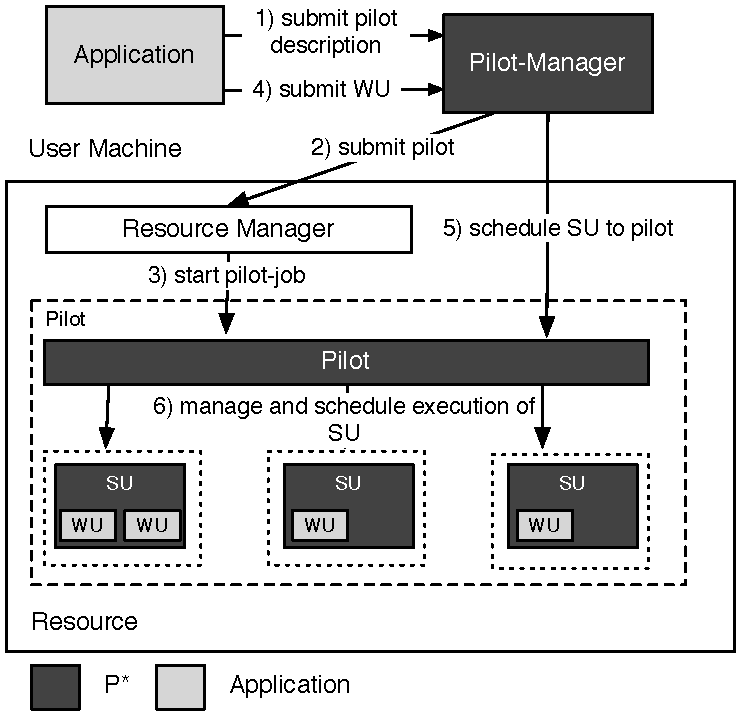
\includegraphics[width=0.43\textwidth]{figures/pstar_model_single.pdf}
    \caption{ \textbf{P* Model: Elements, Characteristics and
        Interactions:} The manager has two functions: it manages 1)
      Pilots (step 1-3) and 2) the execution of \cus. After a \cu is
      submitted to the manager, it transitions to an \su, which is
      scheduled to a \pilot by the PM. The \pilot then schedules the
      \su to an available resource. \alnote{fix caption!}  \upp\upp}
    \label{fig:figures_pstar}
\end{figure}




%\input{sectionII_comments}

\noindent 
\subsection{Elements of the P* Model \upp\upp}
\noindent This sub-section defines the elements of the P* model:

%\alnote{use pilot NOT pilot-job}
\begin{compactitem}
\item \textbf{\pilot \ (Pilot-Compute):} The \pilot is the
  entity that actually gets submitted and scheduled on a resource
  using the resource's RM system. The PJ provides application (user)
  level control and management of the set of allocated resources.

  % and is responsible for the execution of \alwave{SUs/tasks}
  % onto the resource.

  % \alnote{\textbf{The RM assigns a slice of the Resource to the
  %     pilot -- that pilot then acts as RM for that resource slice.}
  %   I think simply equating a pilot with a RM is bit too
  %   simplistic. In a sense it is a application-level resource
  %   manger. Not sure what to do}

\item \textbf{\computeunit \ (\cu):} A \cu \ encapsulates a self-contained
  piece of work (a task) specified by the application that is
  submitted to the \pilotjob framework.  There is no intrinsic notion
  of resource associated with a \cu.

\item \textbf{Scheduling Unit (SU):} SUs are the units of scheduling
  used internal to the P* model, i.e., an SU is not known by or
  visible to an application. Once a \cu has been
  passed into the control of the \pilotjob framework, it is assigned
  to an SU.
  % An SU is created after the submission of
  %   a \cu, i.\,e.\ once a \cu \ has been passed into the control of the
  %   pilot-job framework. 
%  \jhanote{Could we say: Once a \cu has been
%    passed into the control of the pilot-job framework, it is assigned
%    to an SU} \alnote{sounds good. done.}

\item \textbf{Pilot-Manager (PM):} The PM is responsible for (i)
  orchestrating the interaction between the \pilots as well as the
  different components of the P* model (\cus, \sus) and (ii) decisions
  related to internal resource assignment (once resources have been
  acquired by the \pilotjob).  For example, an SU can consists of one
  or more \cus. Further, \cus and \sus can be combined and aggregated;
  the PM determines how to group them, when \sus are scheduled and
  executed on a resource via the \pilot, as well as how many resources
  to assign to an SU.

% the different characteristics of the P* model. It
%   facilitates the coordination between the different P* elements,
%   i.\,e.\ the pilots, \cus and SUs. 
% A PM can e.\,g.\ manage solely one
%   or multiple pilots.

%   For example, the PM has the flexibility to combine and schedule \cus,
%   e.\,g.\ it can determine when a \cu is run and what as well as how
%   many resources it will receive.

\end{compactitem}

% The application itself is not strictly part of the core P* Model.
% The term application generally refers to the upper layer of the
% stack.

An application kernel is the actual binary that gets executed.  The
application utilizes a PJ framework to execute multiple instances of
an application kernel (an ensemble) or alternatively instances of
multiple different application kernels (a workflow).  To execute an
application kernel, an application must define a \cu \ specifying the
application kernel as well as other parameters. This \cu \ is then
submitted to the PM (as an entry point to the
\pilotjob framework), where it transitions to an SU. The PM is then
responsible for scheduling the SU onto a \pilot and then onto a
physical resource.  As we will see in \S\ref{sec:pilot-job-frameworks}, 
the above elements can
be mapped to specific entities in many \pilotjobs in existence and
use; often more than one logical element may be rolled into a specific
entity in a \pilotjob.

% \textbf{Diane Definition of Terms: } The computation consists of
% many worker processes which communicate with one master process (the
% worker processes do not need to share the filesystem nor
% memory). The ensemble of computation is called a run and it consists
% of many tasks which may be executed in parallel. A task is defined
% as a set of parameters which are produced by the RunMaster (running
% on a master node) and consumed by the WorkerAgent (running on a
% worker node).
% 
% from 
% 
% DIANE assumes the master-worker computing model (Fig.
% 1). Client sends job parameters to the Planner which partitions
% the job into smaller tasks executed by the Workers. Integrator
% is responsible for merging the results of task execution and
% sending the final job outcome to the Client.


\subsection{Characteristics of P* Model:\upp\upp}
\label{sec:p_star_elements}

%\jhanote{Why not have Binding as the first characteristics?}

% To understand % the degrees of freedom that any specific pilot-job
% % implementation must constraint as well as
% the functioning of
% pilot-jobs implementation, 
%These characteristics are integral components of the P* Model, in
% Further, these properties are important for the implementation of
% P*.  list several characteristics.
% The way the coordination between the different elements
% is handled is required to understand a PJ implementation.
 
We propose a set of fundamental properties/characteristics that
describe the interactions between the elements, and thus aid in the
description of P* model.

% \alnote{ok} \jhanote{One strategy could be to not define the different
%   types, but just list/enumerate? Akin to Communication. i.e. explain
%   what coordination is for, what is being coordinated, how (the 3
%   types)}

\textbf{Coordination:} The coordination characteristics describes how
various elements of the P* Model, i.\,e.\ the PM, the \pilot, the \cus
and the SUs, interact. A common coordination pattern is master/worker
(M/W): the PM represents the master process that controls a set of
worker processes, the \pilots. The point of decision making is the
master process. In addition to the \emph{centralized} M/W, M/W can
also be deployed \emph{hierarchically}.  Alternatively, coordination
between the elements, in particular the \pilots, can be performed so as
to be \emph{decentralized}, i.\,e.\ without central decision making
point.

%\input{sectionIII-comments}

\textbf{Communication:} The communication characteristics describes the
mechanisms for data exchange between the elements of the P* Model:
e.\,g.\ messages (point-to-point, all-to-all, one-to-all, all-to-one,
or group-to-group), streams (potentially unicast or multicast),
publish/subscribe messaging or shared data spaces.
		
\textbf{Scheduling:} The scheduling characteristics describes the
process of mapping a SU to resources via a \pilot and potential
multiple levels of scheduling. Scheduling has a spatial component
(which SU is executed on which \pilot?) but also a temporal component
(when to bind?). The different scheduling decisions that need to be
made are representative of multi-level scheduling decisions that are
often required in distributed environments.  For example, when should
a SU be bound to a \pilot?  An SU can be bound to a \pilot either before
the \pilot has in turn been scheduled ({\it early} binding), whereas
{\it late} binding occurs if the SU is bound after the \pilot has been
scheduled.  In general, there are multiple-levels at which scheduling
decisions, i.e., resource selection and binding, are made.

The term {\it agent}, although not a part of the P* Model, finds
mention when discussing implementations. For the purposes of this
paper, an agent refers to a ``proxy process'' 
% that either % inside the % pilot-job framework
that has some decision making capability, and could aid the
implementation of one or more of the characteristics of the P* Model
-- coordination, communication, scheduling, within a \pilotjob
framework.  These agents can be used to enforce a set of
(user-defined) policies (e.g.  resource capabilities, data/compute
affinities, etc.) and heuristics.

\subsection{Putting it all together} 
Figure~\ref{fig:figures_pstar}
illustrates the interactions between the elements of the P* model. In
the first step the application specifies the capabilities of the
resources required using a \pilotjob description (step 1). The PM then
submits the necessary number of \pilots in order to fulfill the
resource requirements of the application (step~2). Each \pilot is
queued at the resource manager, which is responsible for starting the
\pilot (step~3). There can be variations of this flow: while in the
described model, the application defines the required resources, the
PM could also decide based on the submitted \cu \ workload whether and
when it submits new \pilots.

%\jhanote{What about the Resource Manager? Is it part of the resource}

The application can submit \cus to the PM at any time (step~4). A
submitted \cu \ becomes an SU, i.\,e.\ the PM is now in control of
it. In the simplest case one \cu \ corresponds to one SU; however,
SUs can be combined and aggregated to optimize throughputs and
response times. Commonly, a hierarchical M/W model for coordination
is used internally: the PM uses M/W to coordinate a set of \pilots,
the \pilot itself functions as manager for the execution of the
assigned SUs.


Scheduling decisions can be made on multiple levels. The PM is responsible for
selecting a \pilot for an SU (step 5). A \pilot is bound to a physical resource
and responsible for managing a particular resource set. Once a SU has been
scheduled to a \pilot, the \pilot decides when and on which part of the resource
the SU is executed.
% \jhanote{Isn't
%   the pilot already bound to a specific resource? Or isn't the pilot
%   bound to a resource and thereby the SU bound to a resource
%   indirectly, and not directly?}  \alnote{Yes, the pilot is bound to a
%   specific resource set, assigning a SU to a pilot means that it can
%   be executed somewhere on this resource set. The pilot decides on
%   which node a SU is run. There can be trivial cases, e.g. DIANE where
%   this decision making does not exist: 1 worker agent == 1 core == 1
%   task. Should we make this more explicit?} \jhanote{Yes -- we
%   could/should make more explicit the fact that pilot is already bound
%   to a resources and assigning a SU to a pilot means it can be
%   executed anywhere on this resource set.} \alnote{refined}
Further, the \pilot also manages the subsequent execution of the SU (step~6).
Again there can be variations of this flow. The above description presents a
typical example of the inner working of a PJ framework, but alternative
implementation of the P* characteristics are possible. PJ frameworks with
decentralized decision making e.\,g.\ often utilize autonomic agents that
accept respectively pull SUs according to a set of defined policies.


\section{Pilot-Job Frameworks\upp\upp}
\label{sec:pilot-job-frameworks}

% \note{OW says: we have this obsession with the term 'framework', but
%   not everything is a framework, e.g., while BigJob and DIANE somewhat
%   resemble a framework, I do not see how Condor can qualify as one.\\
%   For now, I changed the title to 'systems'. If there are no
%   objections, I will make this consistent throughout the
%   text}\alnote{I think we should keep frameworks, I do not see why
%   Condor is not a framework - we also would break consistency with our
%   terms and definitions in section II.}\note{OW says: "In computer
%   programming, a software framework is an abstraction in which
%   software providing generic functionality can be selectively changed
%   by user code, thus providing application specific software." This is
%   definetely not the case for Condor and not really for BigJob. DIANE
%   somewhat resembles a framework.}  \note{OW says: What if we call it
%   Pilot-Job Implementations}

As more applications take advantage of dynamic execution, the
Pilot-Job concept has grown in popularity and has been extensively
researched and implemented for different usage scenarios and
infrastructure. There is a variety of PJ implementations:
Condor-G/Glide-in~\cite{condor-g}, Swift~\cite{Wilde2011},
DIANE~\cite{Moscicki:908910}, DIRAC~\cite{1742-6596-219-6-062049},
PanDA~\cite{1742-6596-219-6-062041}, ToPoS~\cite{topos},
Nimrod/G~\cite{10.1109/HPC.2000.846563}, Falkon~\cite{1362680} and
MyCluster~\cite{1652061}. The aim of this section is to
show that our P* Model can be used to explain/understand some of these
PJ frameworks. In particular we focus on Condor-G/Glide-in, BigJob and DIANE. 


%\jhanote{The aim of this section is to provide a conceptual validation
%  of the P* model by describing/explaining the most commonly used
%  PJ-frameworks and showing how the individual PJ-frameworks map to
%  the P* model, i.e., can be explained by the P* model}


\upp
\subsection{Condor-G/Glide-in\upp\upp}

The Condor project pioneered the concept of Pilot-Jobs by introducing 
the \textit{Condor-G/Glide-In} mechanisms~\cite{condor-g} which allow 
the temporary addition of Globus GRAM controlled HPC resources to a 
Condor resource pool.

In this scenario, the \pilot is exposed as a complete Condor pool that is started 
via the Globus GRAM service of a resource. This mechanism is referred to as Condor
Glide-In. Subsequently, jobs (CUs) can be submitted to the Condor Glide-In pool
using the standard Condor tools and APIs. Condor utilizes a
master/worker coordination model. The PJ manager is referred to as the
Condor Central Manager. The functionality of the Central Manager is
provided by several daemons: the condor\_master that is generally
responsible for managing all daemons on a machine, the
condor\_collector which collects resource information, the
condor\_negotiator that does the matchmaking and the condor\_schedd
that is responsible for managing the binding and scheduling
process. Condor generally does not differentiate between workload,
i.\,e.\ \cu, and schedulable entity, i.\,e.\ SU. Both entities are
referred to as job. However, it supports late binding, i.\,e.\
resources a job is eventually submitted to are not required to be available at
submission time. The scheduler matches the capabilities required by a
\cu to the available resources. This process is referred to as
matchmaking. Further, a priority-based scheduler is used. For
communication between the identified elements Condor utilizes
point-to-point messaging using a binary protocol on top of TCP.

Different fault tolerance mechanisms, such as automatic retries, are
supported.  Further, Condor supports different security mechanisms:
for authentication it integrates both with local account management
systems (such as Kerberos) as well as grid authentication systems such
as GIS. Communication traffic can be encrypted.


\subsection{BigJob: A SAGA-based Pilot-Job Framework\upp\upp}
\label{sec:bigjob_description}
%\terminology{BigJob (BJ) , BigJob-SAGA, BJ implementation, BJ-SAGA, BJ
%  flavors, Amazon EC2, Microsoft Azure, BJ with a Condor Glide-In
%  based backend, BigJob Manager, BigJob agent component, BigJob
%  framework, BigJob pool, extensible scheduler, }


% \jhanote{MUST provide SAGA URL for updated BigJob API and
%   documentation}

% \jhanote{Alternative title: ``BigJob: TROY Pilot-Job'' ?}

% \jhanote{It is CRITICAL to explain why we need to expose the details
%   of multiple atomic BigJobs to the end-user? Remember part of the
%   whole idea of the exercise is, (i) theory: to provide a framework
%   for understanding any differences, (ii) practice: make all these
%   differences go away from the end user!}  \alnote{Since we were not
%   sure about the term ``atomic'', we could also use base bigjob, or
%   core bigjob}



   % 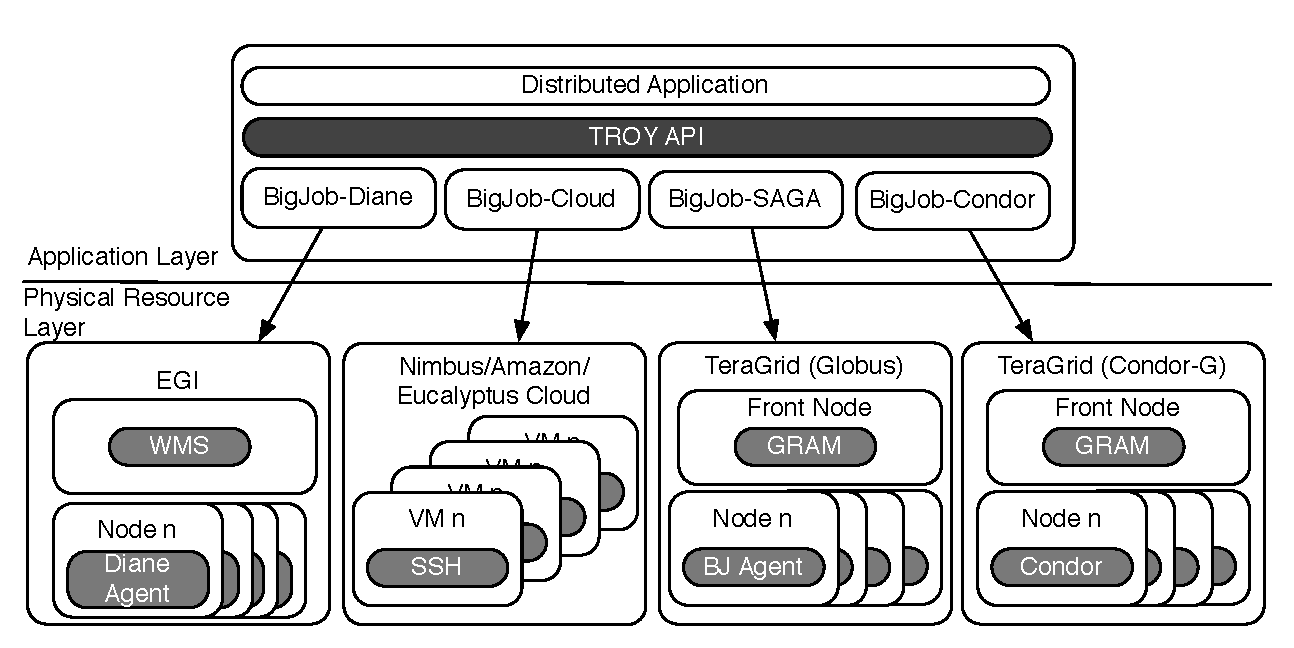
\includegraphics[width=0.3\textwidth]{figures/distributed_pilot_job.pdf}
    % 	\caption{SAGA-based TROY Implementation - BigJob}
    % 	\label{fig:figures_distributed_pilot_job}
    % 	\end{figure}


% General overview of BJ implementations & P* model
%PJ implementations in TROY are called BigJob (BJ)~\cite{bigjob_web}.

BigJob (BJ)~\cite{bigjob_web,saga_bigjob_condor_cloud} is a SAGA-based PJ
framework. BJ has been designed to be general-purpose and extensible. While BJ
has been originally built for HPC infrastructures, such as XSEDE and FutureGrid,
it is generally also usable in other environments. This extensibility mainly
arises from the usage of SAGA as a common API for accessing distributed
resources. SAGA~\cite{saga_url,ogf-gfd-90} provides a simple, POSIX-style API to
the most common grid functions at a sufficiently high-level of abstraction so as
to be independent of the diverse and dynamic grid environments.
By relying on SAGA, BJ is able to run on Globus resources prevailing in HPC
environments, as well as on Cloud resources (such as Amazon EC2 and FutureGrid)
and Condor backends.

% \jhanote{we'll have to unfortunately describe saga briefly in order to
%   make saga-based clear/obvious}\alnote{ok, moved a sentence from
%   Pilot-API section up front.}

\begin{figure}[t]
	\upp\upp\upp\upp
	\centering
	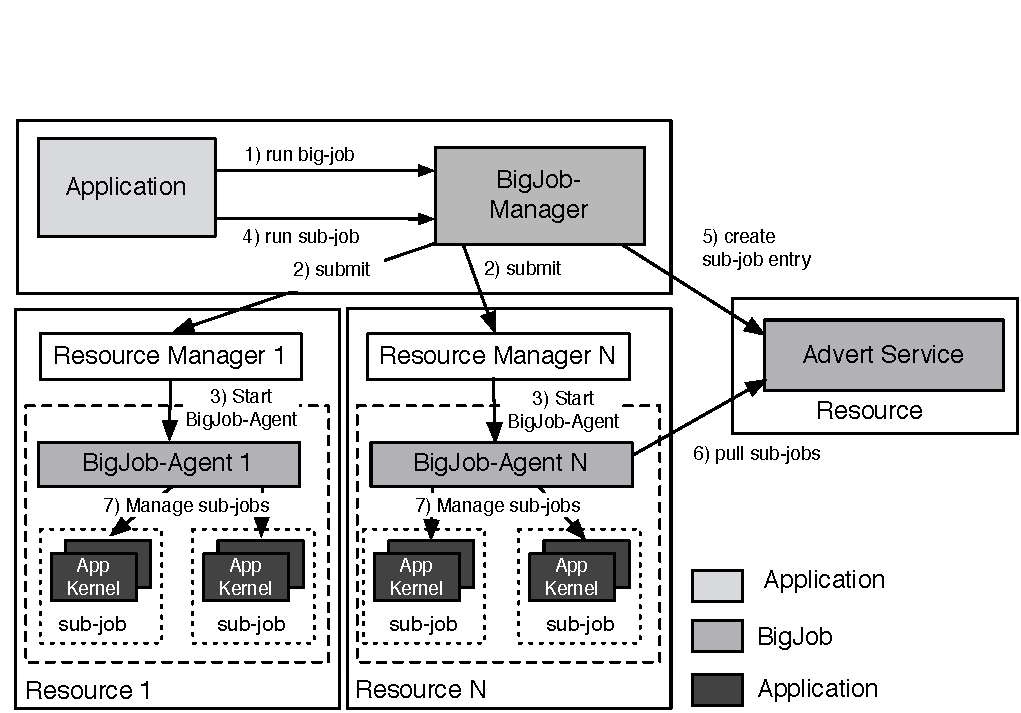
\includegraphics[width=0.45\textwidth]{figures/re_bigjob_interactions.pdf}
	\caption{\textbf{BigJob Architecture and Mapping to P*:} The
          BJ architecture resembles many elements of the P* model. The
          BigJob-Manager is the central Pilot-Manager, which
          orchestrates a set of \pilots. Each \pilot is represented by a
          decentral component referred to as the BigJob-Agent. Sub-job
          -- the \cus -- are submitted via the PM. \cus are mapped 1:1
          to \sus. % \jhanote{Andre, I notice application occurs twice
%             in the box/labels on the bottom right.. please fix}\alnote{done}
        }
	\label{fig:figures_re_bigjob_interactions}
	\upp\upp \upp
\end{figure}


Figure~\ref{fig:figures_re_bigjob_interactions} illustrates the
architecture of BJ and its mapping to P*. The architecture reflects
all P* elements: The BJ-Manager is the Pilot-Manager responsible for
coordinating the different components of the frameworks. The
BigJob-Agent is the actual \pilot that is submitted to a
resource. \cus are referred to as sub-jobs. Internally \cus are mapped
1:1 to \sus.

BJ implements the following characteristic: As coordination model the central
M/W scheme is used: The BigJob-Manager is the central entity, which manages the
actual \pilot, the BigJob-Agent. Each agent is responsible for gathering local
information, for pulling sub-jobs from the manager, and for executing SUs on its
local resource. The SAGA Advert Service is used for communication between
manager and agent. The Advert Service (AS) exposes a shared data space that can
be accessed by manager and agent, which use the AS to realize a push/pull
communication pattern, i.\,e.\ the manager pushes a SU to the AS while the
agents periodically pull for new SUs. Results and state updates are similarly
pushed back from the agent to the manager. Further, BJ provides a pluggable
communication \& coordination layer and also supports alternative c\&c systems,
e.\,g.\ Redis~\cite{redis} and ZeroMQ~\cite{zmq}.
\msnote{The relation between AS and the other pluggables is not clear}

BJ currently uses a simple scheduling mechanism based on an internal queue: each
\cu submitted to the BigJob framework is mapped to a SU. Binding can take place
at submission time (early binding) or delayed in case of multiple \pilots (late
binding). For scheduling, a simple FIFO queue is used (see also
table~\ref{table:pilot-job-comparison}).


% All core BJ are confined to a single resource and don't allow
% neither elasticity nor late binding.

%paragraph on dynamic capabilities
In many scenarios it is beneficial to utilize multiple resources, e.\,g.\ to
accelerate the time-to-completion or to provide resilience to resource failures
and/or unexpected delays. BigJob allows dynamic resource
additions/removals as well as late binding. The support of this feature depends
on the backend used. To support this feature on top of various BigJob
implementations that are by default restricted to single resource use (e.\,g.\
BJ\msnote{Huh?}), the concept of a BigJob pool is introduced. A BigJob pool consists of
multiple BJs (each BigJob managing one particular resource). An extensible
scheduler is used for dispatching \cus to one of the BJs of the pool (late
binding). By default a FIFO scheduler is used.
%  Other backends (such as DIANE
% and Condor) natively support elasticity, but can nevertheless be combined into 
% a % BJ pool.

% \note{OW says: Where is that magic BigJob-Pool and its scheduler? Is there an
% API for that? That's also part of the capabilities provided by
% bigjob-server.}\alnote{The BigJob pool is formerly known as ManyJob. In the
% bigjob/examples directory, there are multiple examples (e.g.
% example\_manyjob\_local.py) that show how multiple BJ can be used concurrently.}

\upp
\subsection{DIANE\upp\upp}

% Coordination and Communication
DIANE~\cite{Moscicki:908910} is a task coordination framework, which
was originally designed for implementing master/worker applications,
but also provides PJ functionality for job-style executions. DIANE
utilizes a single hierarchy of worker agents as well as a PJ manager
referred to as \texttt{RunMaster}.
%Further, there is ongoing work on a multi-master extension.
For the spawning of PJs a separate script, the so-called submitter script, is
required. For the access to the physical resources the GANGA
framework~\cite{Moscicki20092303} can be used.
%GANGA provides a
%unified interface for job submissions to various resource types, e.\,g.\ EGI
%resources or TG resources via a SAGA backend.
Once the worker agents are started they register themselves at the RunMaster.
For communication between the RunMaster and worker agents point-to-point
messaging based on CORBA~\cite{OMG-CORBA303:2004} is used. CORBA is also used
for file staging.

% Binding 
DIANE is primarily designed with respect to HTC environments (such as
EGI~\cite{egi}), i.\,e.\ one PJ consists of a single worker agent with the
size of 1 core.
To use DIANE on HPC environments, a so-called multinode submitter script can be
used: the scripts starts a defined number of worker agents on a certain
resource.
However, \cus will be constrained to the specific number of cores
managed by a worker agent.
By default a \cu  is mapped to a SU; application can however implement smarter
allocation schemes, e.\,g.\ the clustering of multiple \cus into a SU.

%Scheduling
DIANE includes a simple capability matcher and FIFO-based task scheduler.
Plugins for other workloads, e.\,g.\ DAGs or for data-intensive
application, exist or are under development. The framework is extensible:
applications can implement a custom application-level scheduler.


%Other impl. related issues: FT and security
DIANE is as BJ a single-user PJ, i.\,e.\ each PJ is executed with the privileges
of the respective user. Also, only \cus of this respective user can be executed
by DIANE. DIANE supports various middleware security mechanisms (e.\,g.\ GSI,
X509 authentication). For this purpose it relies on GANGA.
Further, DIANE supports fault tolerance: basic error detection and propagation
mechanisms are in place. Further, an automatic re-execution of \cus is
possible.





% \input{sectionIV_comments}
\upp

\begin{table*}[t]
\centering
\begin{tabular}{|p{2.5cm}|p{3cm}|p{3cm}|p{3cm}|p{3cm}|}
  \hline
  \textbf{P* Element} &\textbf{BigJob} &\textbf{DIANE} &\textbf{Condor-G/Glide-in} &\textbf{Swift/Coaster}  \\
  \hline
  Pilot-Manager &BigJob Manager & RunMaster & condor\_master, condor\_collector, condor\_negotiator, condor\_schedd &Coaster Service\\ 
  \hline
  \pilot &BigJob Agent  & Worker Agent &condor\_master, condor\_startd &Coaster Worker\\
  \hline
  \computeunit  \ (CU) &Task &Task &Job &Application Interface Function (Swift Script)\\
  \hline
  \su \ (SU) &Sub-Job &Task &Job &Job\\
% \hline
% Dynamic Resources &no/yes &yes (AgentFactories)\\
\hline
\end{tabular}
\caption{\textbf{Mapping P* elements and PJ Frameworks:} While each PJ framework maintains its own vocabulary, each of the P* elements can be mapped to one (or more) components of the different PJ frameworks.\upp} \label{table:bigjob-saga-diane}
\end{table*}




\upp
\subsection{Swift/Coaster\upp\upp}

Swift~\cite{Wilde2011} is a scripting language designed for expressing
abstract workflows and computations. The language provides among many
things capabilities for executing external application as well as the
implicit management of data flows between application tasks. For this
purpose, Swift formalizes the way that applications can define
data-dependencies. Using so called mappers, these dependencies can be
easily extended to files or groups of files. The runtime environment
handles the allocation of resources and the spawning of the compute
tasks. Both data- and execution management capabilities are provided
via abstract interfaces. Swift supports e.\,g.\ Globus, Condor and PBS
resources.  The pool of resources that is used for an application is
statically defined in a configuration file. While this configuration
file can refer to highly dynamic resources (such as OSG resources),
there is no possibility to manage this resource pool
programmatically. By default a 1:1 mapping for \cu and jobs is
used. However, Swift supports the grouping SUs as well as PJs. For the
PJ functionality the Coaster~\cite{coasters} framework is
used. Coaster relies on a master/worker coordination model;
communication is implemented using GSI-secured TCP sockets. Swift and
Coaster supports various scheduling mechanisms, e.\,g.\ a FIFO and a
load-aware scheduler.

Further, Swift can be used in conjunction with Falkon~\cite{1362680}. Falkon
refers to \pilots as the so called provisioner, which are created using the
Globus GRAM service. The provisioner spawns a set of executor processes on the
allocated resources, which are then responsible for managing the execution of
SUs. \cus are submitted via a so called dispatcher service. Similar to Coaster,
Falkon utilizes a M/W coordination model, i.\,e.\ the executors periodically
query the dispatcher for new SUs. Web services are used for communication.


\subsection{Discussion}

P* provides an abstract model for describing and understanding PJ
frameworks. Table~\ref{table:bigjob-saga-diane} summarizes how P* can
be applied to BigJob, DIANE, Condor-G/Glide-in and Swift/Coaster. While each of 
the frameworks maintains its own vocabulary, all share the common P* elements. 
Table~\ref{table:pilot-job-comparison} summarizes the P* characteristic and 
other properties of these frameworks. While most of these frameworks share many 
properties, such as the M/W coordination model, they differ in characteristics, 
such as the communication model or scheduling.

As we will see further in \S V (Experiments), in spite of a common
Pilot-API each PJ framework has a rather different usage modality;
this is reflective of the fact that typically, PJ frameworks ``evolve
in'' and are ``native to'' specific infrastructure. Native
infrastructure refers to the infrastructure for which a PJ framework
has been primarily developed for and on which infrastructures it is
mainly used, e.g., Condor-G/Glide-in is the native PJ framework of the
Open Science Grid and its use is heavily coupled with WMS; that does
not mean, however, that these frameworks do not work on other
infrastructures.


%Both BigJob and Swift have been
%developed for traditional US cyberinfrastructures, such as
%XSEDE. DIANE is native to EGI e-infrastructure.


% In the next section we will show how these frameworks can be exposed via the 
%Pilot-API.
% In addition to mapping the P* model to different PJ frameworks, we also
% expose BigJob, DIANE and Condor-G/Glide-in through the Pilot-API (see 
% section~\ref{sec:pilot-api}),
% i.\,e.\ the Pilot-API can now be used as a unified abstraction across
% multiple PJ frameworks (see figure~\ref{fig:figures_distributed_pilot_job}).  


\alnote{We haven't introduced the Pilot-API yet This validates (i)
the P* abstractions and (ii) the extensibility of the P*
model.}




% \note{TROY provides a
%   unified API that can be used to expose various PJ frameworks
%   (e.\,g.\ BigJob, DIANE and Condor-G). Further, it enables the
%   concurrent usage of multiple PJ frameworks (see
%   figure~\ref{fig:figures_distributed_pilot_job}). The SAGA inspired
%   approach to TROY's API design --- its SAGA inspired adaptor-based
%   architecture, leverage the design experiences of SAGA, are appealing
%   to the pilot-job user community. Also, the chosen designs enables
%   the easy exchange of PJ implementations and the concurrent use of
%   multiple PJ frameworks. TROY thus functions as common access layer
%   for different PJ frameworks, providing interoperability and
%   portability of PJ applications. To some extent, the TROY API can be
%   considered to be a prototype of a PJ-like API extension to SAGA (see
%   Discussion \& future work, \S\ref{sec:discussion-future-work}).}
% 


% \jhanote{It should probably be Coasters -- which is their notion of a
%   pilot-job.  Just to keep life interesting, they call it head-job and
%   not pilot-job!
%   \url{http://www.ci.uchicago.edu/swift/guides/release-0.92/userguide/coasters.php }}

% \alnote{Swift eval: no standard resource abstraction (SAGA),
%   proprietary language (not Python), TODO: check how coasters work!
%   1 coaster == 1 Condor-G job?}


%\subsubsection*{Other Pilot-Jobs and Conclusion}

% \jhanote{Can we add some structure to these *other* PJ.. this will be
%   ambitious and time-consuming, but if we can, that'll be (i) a great
%   service to the community, (ii) a strong intellectual addition to the
%   paper by virtue of validation of the P*-model}

% \alnote{which are the minimal P* elements and characteristics we
%   should discuss here?}  \jhanote{Andre L: Is this still a
%   valid/live comment/question? If not, should we close}\alnote{can
%   be closed.}

\begin{table*}[t]
\centering
\begin{tabular}{|l|p{2.5cm}|p{2.5cm}|p{2.5cm}|p{2.5cm}|}
	\hline
	\textbf{Properties}
	&\textbf{BigJob} &\textbf{DIANE} &\textbf{Condor-G/Glide-in} &   
	\textbf{Swift/Coaster} \\ \hline

\textbf{Coordination} &Master/Worker  &Master/Worker  &Master/Worker &Master/Worker \\ \hline
	
\textbf{Communication} &Advert Service &CORBA &TCP &GSI-enabled TCP \\ \hline

% \hline
% MPI/Multinode Applications &yes &no (yes with custom implementation of ApplicationWorker)\\
\textbf{Scheduling} &FIFO, custom &FIFO, custom &Matchmaking, priority-based scheduler 
&Load-aware scheduler, \cu  grouping\\

\hfill Binding &\hfill Early/Late &\hfill Late &\hfill Late &\hfill Late\\


\hline
Agent Submission &API &GANGA Submission Script &Condor CLI 
&Resource Provider API\\

\hline

End User Environment &API &API and Master/Worker Framework &CLI Tools &Swift 
script\\ 

\hline

Fault Tolerance &Error propagation &Error propagation, Retries &Error propagation, Retries &Error propagation, retries, replication\\

\hline

Resource Abstraction &SAGA &GANGA/SAGA &Globus &Resource Provider API/Globus CoG 
Kit \\ 

\hline

Security &Multiple (GSI, Advert DB Login) &Multiple (GSI) &Multiple (GSI, 
Kerberos) &GSI\\ 

\hline

% \hline
% Application Interfaces &Big-Job/Sub-job Management &Big-Job/Sub-job 
% Management\linebreak[4] Master/Worker API (\texttt{ITaskScheduler}, 
% \texttt{IApplicationManager}, \texttt{IApplicationWorker}) &&\\

	
\end{tabular}
\caption{\textbf{P* Characteristics and Properties of Different Pilot-Job 
Frameworks:} The properties
in bold-face correspond to the P* characteristics; the other items are general 
properties. The PJ frameworks share many P* characteristics and 
properties, e.\,g.\ the common usage of the M/W scheme or of a 
resource abstraction layer. However, they also differ in aspects, such as  
the coordination model or the used communication framework. 
% \jhanote{Should fix, as this is more than just characteristics...}
% \alnote{done}
\upp\upp}
\label{table:pilot-job-comparison}
\end{table*}

\upp

%
%%%%%%%%%%%%%%%%% SECTION IV - Pilot-API %%%%%%%%%%%%%%%%%%%%%%%%%%%%
%

%\section{An API for the P*  Model\upp\upp}

\section{Pilot-API: A Uniform API to Heterogeneous PJ Frameworks}
\label{sec:pilot-api}
% \alnote{swap 3 and 4? Add mapping of API to PJ framework to API section}

% \terminology{TROY (implementation), P* Model, TROY API, PJ
%   implementation, BigJob, based on SAGA, PJ description, \cu 
%   description, TROY manager class, Condor Glide-In, DIANE, PJ-like
%   API extension) } \alnote{Lead: MS} \alnote{Renaming section and
%   subsections: TROY: A reference implementation of the P*}

In the previous two sections we presented successively the P* Model
and existing Pilot-Job frameworks. Before we present the Pilot-API --
which enables applications to uniformly make use of (heterogeneous)
Pilot-Job frameworks that adhere to the P* Model, we will motivate the
need for such an API.

\subsection{Motivation} 

% 1) similar to workflows
% 2) system level vs. app level interop
% 3) leaky abstractions

% \jhanote{This section should cover threee points: (i) analogy to
%   workflow systems, (ii) different ways to interoperability -- API
%   (SAGA approach) is one, deeper semantic harmonization is the other,
%   (iii) in spite of limitation of API approach - leaky abstractions,
%   it is still useful, and in particular here..}


% Note to Shantenu:
%
%   There exist two ways toward system federation (i) deep integration
%   of systems (system level, interoperation), and (ii) abstract
%   interfaces (application level, integration).
%
% Shantenu, I do agree that the above version is possibly correct, and
% it gives me something to think about :-)  But for the purpose of the
% paper, it may actually complicate things.  For one, our discussion
% of WFs below does not distinguish between interoperation and
% integration, and adding that distinction is adding noise to the text
% (I tried that, it reads aweful).
% 
% More importantly, we user interoperation elsewhere in the text, for
% example when we talk about "Understanding PJ Framework
% Interoperability".  Now, on that level we do not really do interop,
% according to the definition above, but integration (we change none
% of the systems internally, apart from possibly bigjob).  So, we
% would have to change that discussion to integration, which is, while
% being correct I think, complicating the discussion, and also
% somewhat less intuitive for the reader (I think).
% 
% I thus left the definition for now, but please feel free to change
% it, if you feel that the increased correctnes is worth the effort to
% keep the paper consistent.

There exist two ways toward system federation: (A) deep integration of
systems (system level interoperability), and (B) abstract interfaces
(application level interoperability).  Approach (A) requires a certain
level of semantic harmonization between the systems, and is (in
principle and technically) hard to achieve post-facto, even if the
respective systems inherently implement the same abstract model (here:
the P* Model).  While interoperation via an abstract interface (here:
PilotJob API) is a semantically weaker approach than (A), it does
allow for interoperability with minimal (application level)
effort~\cite{saga_bigjob_condor_cloud,saga_gin}.  We thus introduce
the Pilot-API, as an abstract interface to systems implementing the P*
Model.

% The Pilot-API itself was designed to be similar to SAGA in appearance
% and philosophy: it re-uses many of the well defined and standardized
% semantics and syntax.

% \jhanote{place..} SAGA provides a simple, POSIX-style API to the
% most common grid functions at a sufficiently high-level of
% abstraction so as to be independent of the diverse and dynamic grid
% environments.

% The primary design decision for the Pilot-API is its dual nature, one
% part to handle the resource management and another part to deal with
% workload management.

The current state of workflow systems~\cite{nsf-workflow,1196459}
provides a motivating example for the P* Model and the Pilot-API:
Workflow (WF) capabilities and engines are typically tied to specific
tools and infrastructure (e.\,g.\ DAGMan-Condor) and require the
adaption of the application to the WF engine as opposed to the other
way around. Even though many WF systems exist (with significant
duplicated effort), they provide limited means for extensibility and
interoperability.

We are not naive enough to suggest a single reason, but assert that
one important contributing fact is the lack of the right interface
abstractions upon which to construct workflow systems -- had those been
available, it seems very likely that many/most WF engines would have
utilized them (or parts thereof), instead of proprietary solutions.
That would not immediately allow WF implementations to interoperate,
but would make semantic mapping between them significantly simpler,
thus supporting the very notion of interoperation.

The impact of missing interface abstractions on the WF world can be
seen through the consequences of their absence: in spite of
significant effort, WF interoperability at multiple levels remains
difficult if not infeasible.  Significant effort has been invested
towards WF interoperability at different levels -- if nothing else,
providing post-facto justification of its importance.

%\footnote{To be fair: we are not sure if a generic model and/or a
%  generic WF API are achievable {\it on a useful level} -- we think,
%  nevertherless, that our discussion is valid.}


% \jhanote{Somewhere we need to define the different approaches to
%   interoperability. One is via the interface/API; the other is via
%   deeper integration. In the former the lowest common denominator
%   approach is employed. In the latter semantic differences are
%   addressed but at different levels} \alnote{elaborate on
%   SAGA-based approach to interoperability: We use the the API approach
%   to interoperability => talk about approach not api}\jhanote{ditto}
% 
% \note{1) provide expose model 2) api-level interoperability}

% \jhanote{Please elaborate the following} It is also consistent with
% SAGA in that it can support the same underlying job-model...
% \jhanote{ not sure about the relevance of the following sentence:}

However, it is difficult to balance the level of semantic expressivity
for API's designed to work on multiple semantically heterogeneous
systems: defining the API as 'smallest common denominator' is often
too simplifying and misses large numbers of 'edge' use cases; defining
the API as 'greatest common factor' clutters the API with non-portable
semantics, each used by few use cases, thus making the API too
complex~\cite{leaky_abstractions}. 

The Pilot-API in conjunction with the P* Model aims to improve a
similar situation for \pilotjobs. While no single solution can address
all levels nor the entire spectrum of applications, the Pilot-API
exposes effective abstractions that can hide environmental complexity,
supplement the incompleteness and lack-of-extensibility of many tools,
and generalize customized run-time solutions for a broad range of
applications.  The Pilot-API uses the Pareto principle as a guideline
for a balanced abstraction level.

% \amnote{according to Shantenu, 'abstraction' is over-used in the text
% above.  I changed some occurences, but more remain which I am not sure
% how to replace without increasing noise.}

% MS: commented out the next session as it talks about the runtime system
% The pilot-job capabilities in TROY are provided by different PJ
% frameworks that are integrated into the TROY runtime system via
% adaptors. For this purpose, TROY defines a Capability Provider
% Interface (CPI) that must be implemented by the adaptors of the
% underlying pilot-job frameworks. This architecture also enables the
% concurrent usage of multiple PJ frameworks.  \jhanote{NO mention of
%  CPI should occur}

\begin{figure}[t]
    \centering
\upp
    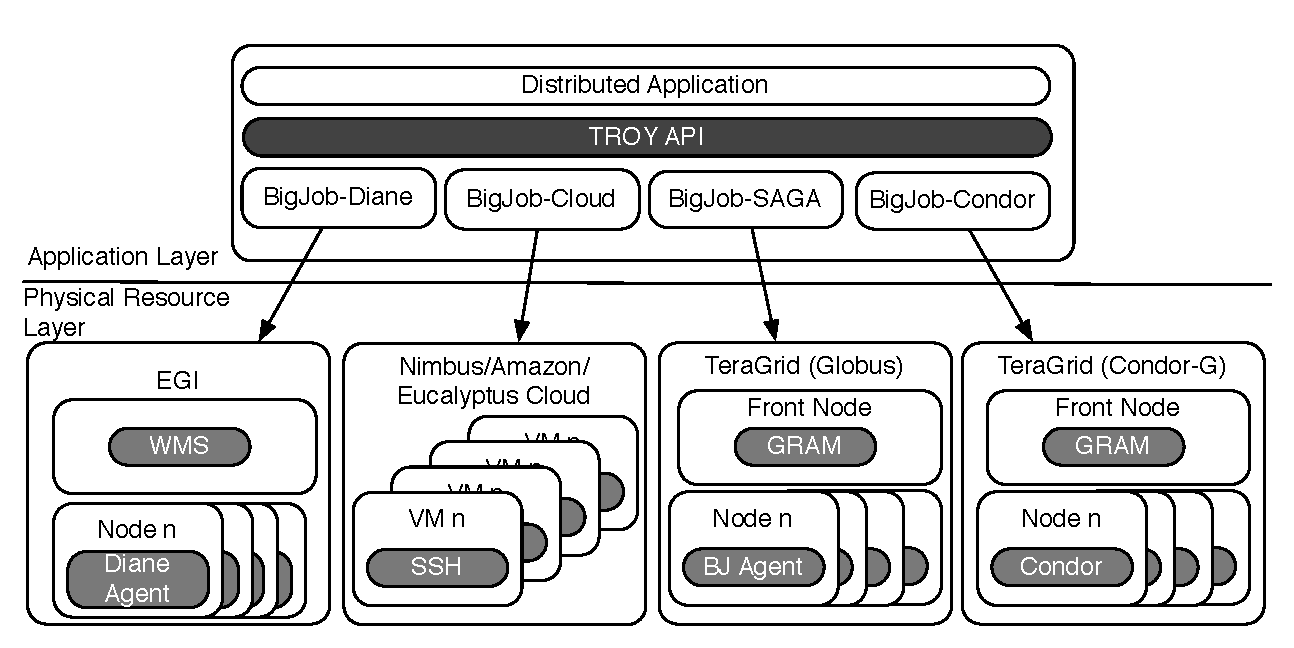
\includegraphics[width=0.48\textwidth]{figures/distributed_pilot_job.pdf}
    \caption{\textbf{Pilot-API and PJ frameworks:} The Pilot-API provides 
      a unified interface to utilize the native Pilot-Job capabilities of
      different infrastructures, e.\,g.\ BigJob for XSEDE/Cloud
      resources, DIANE for EGI and Condor for OSG resources.
%       It also enables the concurrent usage of these infrastructures.
	\upp\upp\upp}
    \label{fig:figures_distributed_pilot_job}
\end{figure}

% \begin{figure}[t]
% 	\upp
% 	\centering
% 		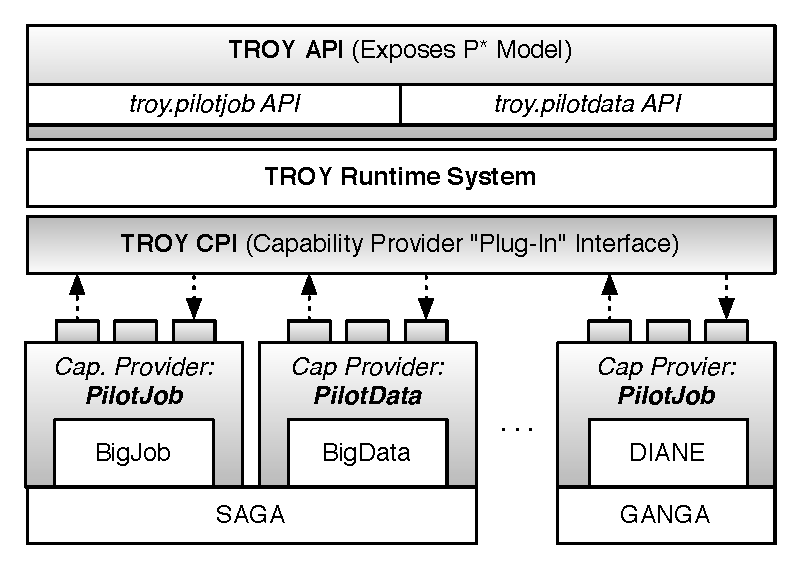
\includegraphics[width=0.45\textwidth]{figures/TROY_arch.pdf}
%                 \caption{\textbf{TROY -- An API and Runtime System for
%                     the P* Model:} TROY provides an API for managing
%                   PJs and PDs. BigJob and BigData are realizations of
%                   the actual PJ and PD functionality. BJ and BD rely
%                   on SAGA for implementation of the PJ/PD.
% 	\label{fig:figures_pstar_troy}
% 	\upp\upp
% \end{figure}

\subsection{Understanding the Pilot-API}

The Pilot-API supports two different usage modes i) it provides a unified API to
various PJ frameworks (e.\,g.\ BigJob , DIANE and Condor-G/Glide-in), and ii)
it enables the concurrent usage of multiple PJ implementations.

The Pilot-API classes and interactions are designed to reflect the P*
elements and characteristics.
% Table~\ref{table:pstar_elements} summarizes the mapping of P* elements and the
% Pilot-API.
As defined by P*, a \cu represents a primary self-containing piece of work that
is submitted through the Pilot-API. 
At the API boundary a \cu transitions to a SU, which functions as internal unit
of scheduling.

The API follows object-oriented design principles and exposes the primary
functionality of the Pilot-Manager using two classes: the \texttt{PilotService}
for the management of pilots and the \texttt{ComputeUnitService} for the
management of \cus. 

Figure~\ref{fig:figures_pilot_api_flow} shows the interactions between the
P* elements. The Pilot-API \footnote{We use Python syntax for describing
the Pilot-API.}
decouples workload management and resource
scheduling by exposing two separate services: The
\texttt{PilotService} (PS) and \texttt{ComputeUnitService} (CUS). The
PS serves as a factory for instantiating pilots. Also, the PS can be
used to query the PS for currently active pilots.  A
\texttt{Pilot} object is returned as result of the
\texttt{create\_pilot()} method of the PS (step 1).

Analogous to job creation in SAGA, the instantiation of the \texttt{Pilot}
object is done by using a \texttt{PilotDescription}. The description can be
reused and has no state, while the \texttt{Pilot} instance has state and is a
reference for further usage.

\lstset{
language=Python,
frame=single,
captionpos=b,
stringstyle=\ttfamily,
basicstyle=\scriptsize\ttfamily
}

\noindent\begin{minipage}{0.47 \textwidth}
\begin{lstlisting}[caption={\textbf{Pilot Creation:} Instantiation of a Pilot Service using a Pilot Description.}, label={lst:ps_creation}]
ps = PilotService()
p_desc = PilotDescription()
p_desc.total_core_count = 8
p = ps.create_pilot('gram://queenbee', 
                          p_desc, 'bigjob')
\end{lstlisting}
\end{minipage}

The \texttt{Pilot} object represents a pilot instance and allows the 
application to interact with a pilot, e.\,g.\ to query its state or to cancel 
it. The process of Pilot creation is depicted in step 1-2 of 
figure~\ref{fig:figures_pilot_api_flow} and in listing~\ref{lst:ps_creation}.

Listing~\ref{lst:cus_creation} shows the creation of a CUS.
Having instantiated a \texttt{ComputeUnitService} object, PS objects can be
added and removed at any time. This enables applications to respond to dynamic
resource requirements at runtime, i.\,e.\ if peak demands arise an application
can request additional resources; if resources are not required anymore, they
can be released.

\noindent\begin{minipage}{0.47 \textwidth}
\begin{lstlisting}[caption={\textbf{ComputeUnitService Creation:} Instantiation
of a \texttt{ComputeUnitService} using a reference to the
\texttt{PilotService}.}, label={lst:cus_creation}]
cus = ComputeUnitService()
cus.add(ps)
\end{lstlisting}
\end{minipage}

\noindent\begin{minipage}{0.47 \textwidth}
\begin{lstlisting}[caption={\textbf{ComputeUnit Submission:} Instantiation and 
	submission of a \texttt{ComputeUnitDescription}.}, label={lst:submission}] 
cud = ComputeUnitDescription()
cud.executable = '/bin/bfast'
cud.arguments = ['match', '-t4', '/data/file1']
cud.total_core_count = 4
cu = cus.submit(cud)
\end{lstlisting}
\end{minipage}

% \lstset{
% caption={\textbf{WorkUnit Submission:} Instantiation and Submission of a \texttt{WorkUnitDescription}.\label{lst:submission}}
% }

The \texttt{ComputeUnitService} is responsible for managing the execution of
\cus.
Regardless of the state of the PS, applications can submit \cus to a
\texttt{ComputeUnitService} at anytime (listing~\ref{lst:submission} and step 3
in figure~\ref{fig:figures_pilot_api_flow}). 
Once the \texttt{ComputeUnitService} becomes responsible for a \cu, the \cu
transitions to an SU.
SUs are internally processed (they e.\,g.\ can be aggregated) and are then scheduled to the Pilot-Job Framework (step 4). 
The PJ framework is responsible for the actual execution of the SU on a
resource.
Note that multiple levels of (hierarchical) scheduling can be present, commonly
a SU is scheduled inside a PJ framework and the model allows it to be present
in multiple layers.



% In figure~\ref{fig:figures_pilot_api_flow} the flow of a simple execution scenario is
% displayed. The Pilot Job Service and the Work Unit Service are already
% instantiated. The application requests the Pilot Job Service to create a new
% pilot-job (step 1), the Pilot Job Service will pass the request on to the
% relevant adaptor (step 2), which will eventually launch the pilot-job on a
% resource using a pilot-job framework (step 3). At this stage there might be a
% pilot-job already available, or the request can still reside in a queue
% somewhere. Regardless of the state of the pilot-job, the application can submit
% a work unit to the Work Unit Service (step 4). The Work Unit Service remains
% responsible for keeping track of the Work Unit during its lifetime. Based on the
% heuristics or policies the WUS decides on a potential aggregation of SUs. The SU 
% is then forwarded to the Scheduler (step 5). The Scheduler will schedule SUs to 
% an appropriate adaptor that represents a capable resource (step 6). Finally, the
% adaptor will submit the SU to the PJ framework which will
% take care of the actual execution on a resource. Note that multiple levels of 
% (hierarchical) scheduling can be present. Inside
% TROY there is already scheduling taking place inside the Work Unit Service. 
% Additionally, the underlying PJ framework can conduct its own scheduling.


Each \texttt{ComputeUnit} and the \texttt{Pilot} object is associated with a
state. The state model is based on the SAGA job state
model~\cite{ogf-gfd-90}.
\note{OW says: Why? IMHO the GFD.90 state model has some serious flaws, like
the absence of a 'Waiting' state.} \amnote{What is a waiting state?
Who is the waiting on what?}
\msnote{I would actually prefer to model it after the BES state model, in practice that is what I do in TROY.}
Applications can query the state using the \texttt{get\_state()} method or they
can subscribe to state update notifications.

Finally, an application can have any number of \ps or ComputeUnit
Services.  Multiple PilotServices can be associated to a ComputeUnitService,
and a PilotService can be associated to multiple ComputeUnitServices. A
ComputeUnitService can manage multiple ComputeUnits, but a ComputeUnit can only
be managed by one ComputeUnitService. So can a PilotService manage multiple
Pilots, but can a Pilot only be managed by one PilotService.


\begin{figure}[t]
	\centering
		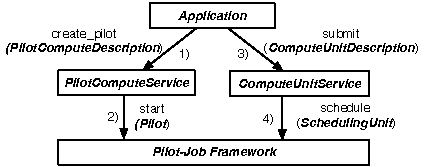
\includegraphics[width=0.47\textwidth]{figures/pilot-api-flow.pdf}
	\caption{\textbf{Control Flow Pilot-API and PJ Frameworks:} The functionality    of pilot-jobs are exposed 
	using two primary classes: The \texttt{PilotService} for the management 
	of pilots, and the \texttt{ComputeUnitService} for the management of \cus.
    \alnote{figure needs attention.}
	}
	\label{fig:figures_pilot_api_flow}
\end{figure}

%\begin{table}[t]
%	\centering
%\begin{tabular}{|l|l|}
%\hline
%\textbf{Pilot} &PJ framework\\
%\hline
%\textbf{\cu } &\cu \\
%\hline
%\textbf{SU} &SU\\
%\hline
%\textbf{Pilot-Manager} & PilotService/ComputeUnitService\\
%\hline
%\end{tabular}
%\caption{Mapping of P* and the Pilot-API\upp\upp
%\msnote{\\\\I find this a rather unuseful table and can be axed if you ask me}
%}\label{table:pstar_elements}
%\end{table}



\section{Experiments and Results\upp\upp}
\label{sec:exp_res}

In this section we analyze the performance and scalability of
different PJ frameworks.  \msnote{Do we?} It is important to note that our experiments
do not try to identify the ``best'' or ``fastest'' PJ framework, as
this is dependent on different factors, e.\,g.\ particularly the
infrastructure used -- the experiments are conducted on different
production (XSEDE, EGI, OSG) and research (FutureGrid) infrastructres. 

As discussed in \msnote{section?} \ref{sec:pilot-job-frameworks}, the investigated PJ frameworks can be mapped to
the P* model, which enables their collective usages via the Pilot-API.
In section~\ref{sec:pj_performance} we investigate the performance and
scalability of coordination in BigJob and DIANE, executing thousands
of tasks but with zero workload. \jhanote{Andre L, please check} In
section~\ref{sec:fg-xsede-osg-egi} we show the effectiveness of our
approach (Pilot-API/P* Model) by executing {\it real application
workloads} -- in this case a genome alignment tool -- on
multiple distinct production infrastructures.  Further, we demonstrate
interoperability by using multiple PJ frameworks concurrently on
multiple infrastructures using the Pilot-API -- see
section~\ref{sec:experiment-interop}.



% \jhanote{Need a simple description of experiment   configuration}.
% \alnote{Is it ok to just describe the configuration on high-level in the 
% introduction and do this in detail in the sub-sections?}\jhanote{yes}

% \alnote{this paragraph is redundant to B and C? Alternative we can move
% stuff from there to here.}
% For purposes of validation, demonstration and performance
% measurements, we use the Pilot-API to marshall different PJ
% frameworks...  The experiments are conducted on different
% production (XSEDE, EGI, OSG) and research infrastructures
% (FutureGrid).

% \jhanote{Need to provide details of the application} 
% \alnote{Is it ok to do this in subsection B and C?}\jhanote{yes} 

%(with SAGA/PBS and SAGA/Condor) and DIANE in a genome sequencing
%application scenario.



% \amnote{Someone please check the above statement for sanity!}
% \alnote{What's a concertation?}  \amnote{wiktionary says: "A form of
%   dialogue and co-decision, implying the mutual exchange of
%   information, open discussion and knowledge sharing, and the
%   signature of operational agreements between public administrations
%   and/or with representatives of the private sector."  Basically
%   means in our context 'in a coordinated way, in
%   combination'.}\jhanote{Would `` collectively'' be a better
%   description?}

\subsection{Understanding Coordination in PJ Frameworks\upp\upp}
\label{sec:pj_performance}

Different PJ implementation follow different design objectives -- that
also reflects in the designs of their communication \& coordination
(\cc) sub-systems.  The primary barrier for performance and
scalability is not the \cu  submission, but the internal coordination
of the elements of a PJ implementation. There are many factors that
influence the overall performance, e.\,g.\ the degree of distribution
(local (LAN) vs. remote (WAN)), the communication pattern (1:n versus
n:n) and the communication frequency. In the following we investigate
the impact of different \cc related factors on the overall
performance and scalability of PJ systems.  We evaluate different
BigJob \cc configurations, and compare and contrast them with DIANE.

BigJob's \cc was originally based on a shared, centralized data space
('tuple space'), the SAGA Advert Service~\cite{saga_advert}.  The
communication between all components is done via this shared data
space, which decouples BJ-Manager and BJ-Agent and allows both
entities to operate at their own pace, optimizing the overall
throughput.  A particular issue during distributed runs is the latency
between the application and the (remote) Advert Service. Another
challenge is that this design introduces a potential
single-point-of-failure and scalability bottleneck if the centralized
data space is not carefully designed and operated.

BigJob also provides two alternative c\&c sub-systems:
Redis~\cite{redis} and ZeroMQ~\cite{zmq}. Redis is a lightweight
key/value store, which can be deployed locally, or in a distributed,
fault tolerant way. Redis is used in a similar way as the Advert
database, i.\,e.\ all communication between BJ-Agent and BJ-Manager is
channeled through it. In contrast, the ZeroMQ sub-system utilizes a
client-server architecture, which is similar to the CORBA-based \cc
sub-system of DIANE -- in this architecture, the PM maintains the
overall state. Clients connect to the PM to request new SUs or to
report state updates. An advantage of this architecture is that it
does not require a separate infrastructure deployment for the \cc
sub-system.
%
% While the BJ-Manager can be deployed remotely from the BJ-Agent, in
% most cases this will not be the case, i.\,e.\ the communication
% between BJ-Manager and BJ-Agent is mostly local communication. 
% 
% AM: I do not understand the above, really: following fig. 2, the
% agent *is* remote to the manager?
%
Both the data space and the ZeroMQ client-server \cc sub-systems can be
combined with a publish/subscribe mechanism, i.\,e.\ instead of
polling, an agent can receive notifications when a new SU arrives.
\amnote{AL: please check the tex-comments in the paragraph above.}

For our \cc evaluation, we conducted several experiments on
FutureGrid~\cite{fg}. To evaluate overall performance, throughput and
scalability, we executed a different number of very short running
(i.\,e. zero workload) \cus on Alamo and Sierra, utilizing up to 128
cores concurrently.  This enables us to focus on the overhead induced
by the PJ framework and the \cc subsystem. Each experiment is
repeated at least 10 times.

\amnote{'128 cores concurrently' - for each cus?  Because, the graphs
go up to 2048 cores.  Also, how would the number of cores/cus
influence the \cc?  It should not, as communication is per cus, not
per CPU core?}

% \jhanote{Need to motivate testing of c\&c sub-system better: There are
%   many barriers to interoperability and performance. primary barrier to
%   performance is not \cu  submission or SU scheduling to PM, but the
%   fundamental limitation of scalability of coordination -- with
%   increasing number of \cu /SU.  Establish tradeoff between distributed
%   vs local coordination. e.g., It is easy to get consistency but has
%   overhead.  Easy to get performance but difficult to get
%   consistency. Thus we opt for centralized / persistent point. But how
%   does this single point-of-coordination behave with increasing number
%   of connections? } \alnote{hopefully addressed most points in paragraph above}

% \begin{figure*}[htbp]
% 	\centering		
% 	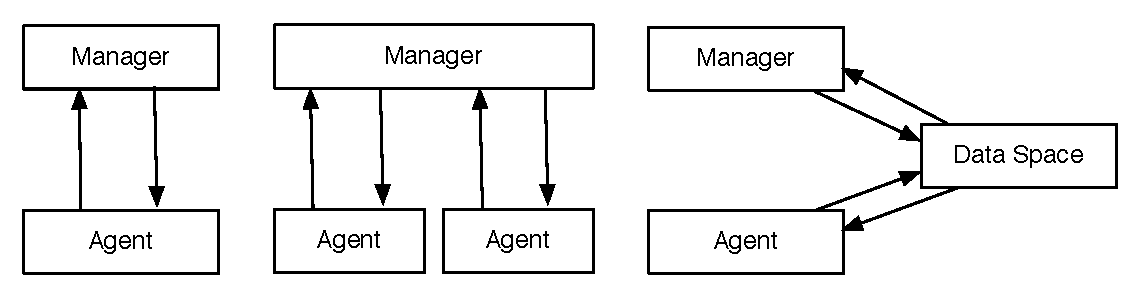
\includegraphics[width=0.8\textwidth]{figures/coordination-schemes.pdf}
% 	\caption{\textbf{Coordination \& Communication:} The primarily used 
% 	coordination pattern is the utilization of a request/response server 
% 	(left, middle). In the data-space model (right) all application components 
% 	are connect to a central data-space. This architecture decouples manager 
% 	and agent allowing both to operate on its own pace.}
% 	\label{fig:figures_coordination-schemes}
% \end{figure*}

% Figure~\ref{fig:figures_coordination-schemes} illustrates different
% coordination schemes. 

% Most pilot-jobs utilize the master-worker \jhanote{M-W for what?}
% pattern commonly implemented on basis of a simple request/response
% architecture, i.\,e.\ the \jwave{agent} sends a request for work
% packages to the master, which replies with a \cu . 

% \jhanote{Are we talking specific implementation, i.e., TROY? If so we
%   should not say ``A'' manager but ``The Pilot-Manager''? Also the previous
% sentence should not talk about most pilot-jobs, if we've already started
% talking about TROY!!} \alnote{hopefully fixed.} 

% A manager
% can manage a single agent (e.\,g.\ BigJob) or multiple agents
% (e.\,g.\ DIANE). 


\begin{figure}[htbp] 
 \centering
 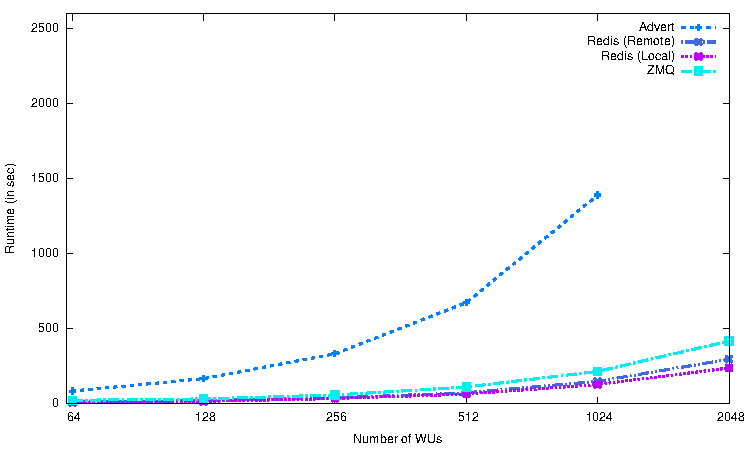
\includegraphics[width=0.49\textwidth]{perf/bigjob-varying-wus-alamo.pdf}
 \caption{\textbf{BigJob and DIANE Performance (1):} The 
  time-to-completion for $n$ \cus scales linearly
  in most cases, i.\,e.\ the coordination overhead imposed by the BJ is 
  minimal.
  \amnote{only the DIANE graph is linear, AFAICS}
  \upp\upp}
 \label{fig:perf_bigjob-varying-wus} 
\end{figure}

Figure~\ref{fig:perf_bigjob-varying-wus} illustrates the performance
and scalability of different BigJob configurations and DIANE with
respect to the number of \cus. Clearly, the \cc sub-system has a great
impact on the overall performance: the Redis backend shows the best
performance for small \cu counts. \amnote{That is very hard /
impossible to see in the graph!} The difference between local and
remote coordination is moderate (about 20\,\%). While ZeroMQ is very
fast and lightweight, it requires a careful implementation, in
particular concerning synchronization and throughput optimization. The
overall performance is slightly worse than for Redis. The Advert
Service currently has some limitations which will be discussed later.
DIANE shows a higher startup overhead, which is particularly
observable for smaller \cu  numbers. \amnote{again, hard to see in
graph!} However, the runtime increases only slightly (about 10\,sec)
when going from 64 to 2048 \cus. One reason is that DIANE aggregates
SUs: for 2048 \cus only a single task description is created, which
the framework efficiently distributes to its agents. BigJob in
contrast maintains a separate description for each \cu. 
% At the investigated scales, the single manager does not represent a
% bottleneck with respect to the processable \cu  numbers. Further,
% the TROY manager introduces another hierarchy-level which can
% further enhance the overall scalability.

Figure~\ref{fig:perf_bigjob-varying-cores} illustrates the performance
scalability with respect to the number of cores. \amnote{cores of
what?  per pilot, per cus?} In particular, the Redis (Local)
configuration show an almost linear scalability up to 128 cores. The
Redis (Remote) setup again imposes some overhead (about 14\,\%). ZeroMQ
performs very well with lower core counts; with larger core counts the
runtimes increase, indicating a potential scalability bottleneck. DIANE
shows, in particular for lower core counts, a longer runtime, again due
to the higher startup overhead.  With higher core counts DIANE behaves
similar to BigJob/ZeroMQ, showing a greater increase of the overall
runtime. This increase can likely be attributed to the single central
manager in the client-server architecture. As in the last experiment,
the Advert \cc sub-system showed a significantly lower performance.
\amnote{the text above does not explain the 'constant workload of 4
cus' -- what does that mean?  Whenever one cus of the is done, a new
one is submitted?  Or are there just 4 cus with long runtimes?  I am
not really sure what exactly is measured here...}

\begin{figure}[htbp] 
 \centering
 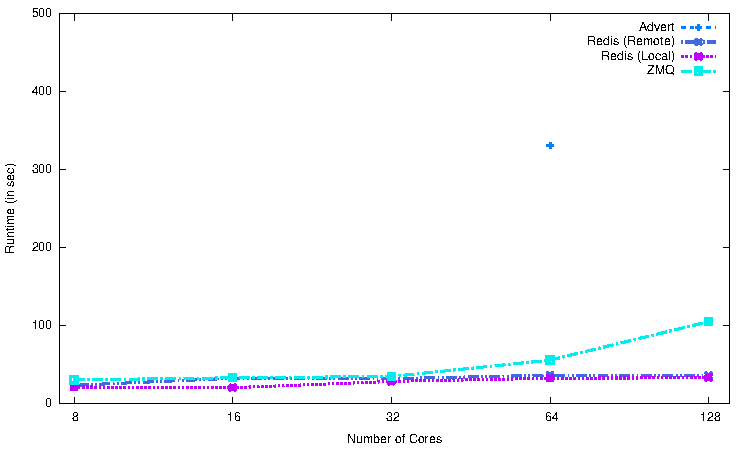
\includegraphics[width=0.49\textwidth]{perf/bigjob-varying-cores-alamo.pdf}
 \caption{\textbf{BigJob and DIANE Performance (2):}  The
  runtime of a constant workload of 4 \cus 
  increases only slightly up to 128 cores. In particular, the Redis backend shows
  an almost linear scalability achieving a throughput of up to 4 \cus/sec. }
 \label{fig:perf_bigjob-varying-cores} 
 \upp\upp
\end{figure}

The Advert Service implementation currently shows some performance
limitations, mainly caused by the prototypical nature of its
implementation.  Further, it must be noted that the Advert Service was
deployed remotely (mainly due to deployment constraints). Even so, the
discrepancy between Advert Service and Redis (Remote), which has been
deployed on the same remote network, is significant. A reason for that
is the used remote access protocol, which is basically the native
remote PostgreSQL database protocol, which is not optimized for WAN
connections.
%
% \jhanote{It is not clear why REDIS and ZeroMQ are not susceptible to
% access over WAN delays/latency?}\alnote{included a comparison note
% to Redis Remote. We can't compare it to ZMQ since we use only local
% communication in this case}
%
Transactions e.\,g.\ are very latency sensitive and require several
roundtrips.  Further, the API is based on a hierarchical namespace,
which does not easily map to relational databases -- in deeply nested
namespaces exhibit an insufficient query and update performance. In
contrast, data is stored in memory for Redis and ZeroMQ, which
partially explains the significant performance gains.

\upp

\subsection{Characterizing PJ Frameworks on Production Infrastructure\upp\upp}
\label{sec:fg-xsede-osg-egi}

\msnote{FG is not production infra}\jhanote{it is classified as
  ``production research'' infrastructure! go figure..!!}

\subsubsection*{Production Infrastructure} To validate the developed
abstractions, we conducted a series of experiments on various
production infrastructure. We executed BFAST~\cite{bfast2009} -- a
genome alignment tool -- using three different PJ frameworks
(BigJob, DIANE and Condor) on XSEDE~\cite{xsede},
FutureGrid~\cite{fg}, EGI~\cite{egi} and
OSG~\cite{1742-6596-78-1-012057}.

Specifically, we utilized the following resources: XSEDE: Kraken (1.17
PFlop Cray XT5 / 9,408 nodes / 112,896 cores / Torque) and QueenBee
(Linux Cluster / 668 nodes / 5,344 cores / PBS); FutureGrid:
India (Linux Cluster / 108 nodes / 864 cores / PBS); European Grid
Initiative (EGI): Resource federation of 364,500 cores.;
OSG: Condor pool (via the \textit{Engage} VO, Glide-In WMS,
20,000 Glide-Ins\footnote{Glide-In WMS is a software system built on
top of Condor-G/Glide-in which can, based on the current and expected
number of jobs in the pool,  automatically increase or decrease the
number of active Glide-Ins (\pilots) available to the pool.  While the
average number of active Glide-Ins on OSG is around 20,000, more than
40,000 Glide-Ins can be active and available for job execution during
peak load.}.

 
%\jhanote{I would even introduce a sub-subsection on production
%  infrastructure used. That would enable us to keep Pilot-API/BigJob
%  specific details separate from infrastructure details. E.g., say
%  what is XSEDE? Say what is OSG? Thoughts?}  \alnote{good
%  idea. started to restructure section}


%\note{OW says: That would be the case if we use Condor-G. The machines
%is belhaven-1.renci.org - a Globus/PBS cluster that accepts Condor jobs.\\
%So the OSG is a peculiar beast. My current understanding is, that it consits 
%of a bunch of HPC clusters with a Globus frontend. OSG uses an automated 
%Glide-in WMS service that starts glide-ins via Condor-G on these clusters.
%The glide-ins are aggregated and presented to the OSG (HTC) user as a 
%standard condor pool for HTC jobs. While using OSG through condor seems 
%to be a popular mode of operation, it is possible to access any of the 
%OSG-member clusters via Condor-G and through Globus directly. As far as I
%understand, this is the preferred mode for running HPC (multi-core) 
%applications.\\
%This raises two important questions: does it make sense it all to use
%BigJob with the OSG condor pool? We would end up with one BJ agent per
%condor job which represents one core, which would just add a lot of overhead and
%no benefits. Using OSG via Condor-G or even Globus would allow us to
%take advantage of larger reservations, e.g. one BJ agent that manages
%128 cores.\\
%While it would make sense for TROY to implement a native Condor 'backend'
%that doesn't use another layer of 'agents' and master/worker advert 
%mechanisms, I don't think that this makes sense for BigJob. Depending on 
%what we want to show, I propose that we use BigJob with Globus (we now that 
%it works) on OSG. While this doesn't show pilot job interoperabiltiy
%(which his hard to achieve without TROY anyways), it still shows cross-grid
%interoperability.}


% To manage the genome sequencing workflow we use
% theDARE~\cite{dare-tg11-gateways} framework that has been built on
% top of TROY.

\subsubsection*{Experimental Configuration}

%\jhanote{Experimental Configuration = Infrastructure used, specific
%  machine (on XSEDE and FG) and resources configuration + PJ Framework
%  employed.}

We define an experimental configurations as a set comprised of the
production infrastructure used, the specific machine/resource
configuration, and the utilized PJ framework.
%\amnote{should mention here that the PJ frameworks are utilized via
%TROY, and implementation of the Pilot-API, and add a forward
%reference?  Otherwise, how can we motivate that this is validating the
%API?}

The investigated workload consists of of 128 \cus. Each \cu executes a
BFAST matching process, which is used to find potential DNA sequence
alignments. The scenario requires about 7\,GB input data: 1.7\,GB for
the reference genome and index files, and 5.4 GB \textit{short read} 
files, generated by a DNA sequencing machine (32 files,
1.68\,GB each). We run the experiment on four different
configurations: (i) BigJob+Pilot-API/XSEDE, (ii) BigJob+Pilot-API/FutureGrid, 
(iii) Condor+Pilot-API/OSG, (iv) DIANE+Pilot-API/EGI. 
As discussed in section~\ref{sec:pilot-api}, the Pilot-API provides a 
unified way to access the different native PJ capabilities for all
three PJ frameworks, i.\,e.\ BigJob, DIANE and Condor. 


% .  \onote{Not quite sure why i,iii,iv say 'only' and 'ii'
%   doesn't. what about interop configurations?}

% To achieve interoperability, we have developed a Pilot-API to
% interface with all three PJ frameworks, i.\,e.\ BigJob, DIANE and
% Condor. The Pilot-API provides a unified way to access the different
% native PJ capabilities.

% For the experiments we rely both on the native PJ APIs, in
% particular the BJ API, and the Pilot-API.

BigJob uses its PBS/SSH plugin to access India/FutureGrid, and the
SAGA-Torque adaptor to access Kraken/XSEDE. For OSG, we utilize SAGA
(wrapped in the Pilot-API) and the SAGA-Condor adaptor to interface 
directly with OSG's dynamic GlideIn-WMS resource pool.  Further, we 
utilize DIANE on EGI. \msnote{more on EGI later ...} 
%On the XSEDE, Kraken is used with up to 512 cores concurrently.
%\amnote{why is the corecount mentioned for Kraken, and not the others?}

In each scenario, 128 \cus are defined and submitted to the Compute
Unit Service.  Each BFAST \cu requires 1 core; depending on the
resource and resource assignment policy a different number of cores
maybe assigned for each BFAST \cu, e.\,g.\ on Kraken 4 cores are
reserved for each \cu. Each \cu is associated with a set of input
files which is pre-staged in configuration (i) and (ii). For the HTC
infrastructures EGI and OSG (configurations (iii) and (iv)), these
file are transferred before running each \cu. \jhanote{how does his
  differe from pre-staging?}

% Having submitted the 128\,\cus, the benchmark application can use
% the Compute Unit Service of the Pilot-API to monitor the \cu's
% state.  
% AM: the above is not relevant here -- only interesting in the API
% description section
\amnote{I don't understand: "Each BFAST \cu requires 1 core", but "on
Kraken 4 cores are reserved for each \cu"???}\jhanote{fixed}

\begin{figure}[t]
 \centering
 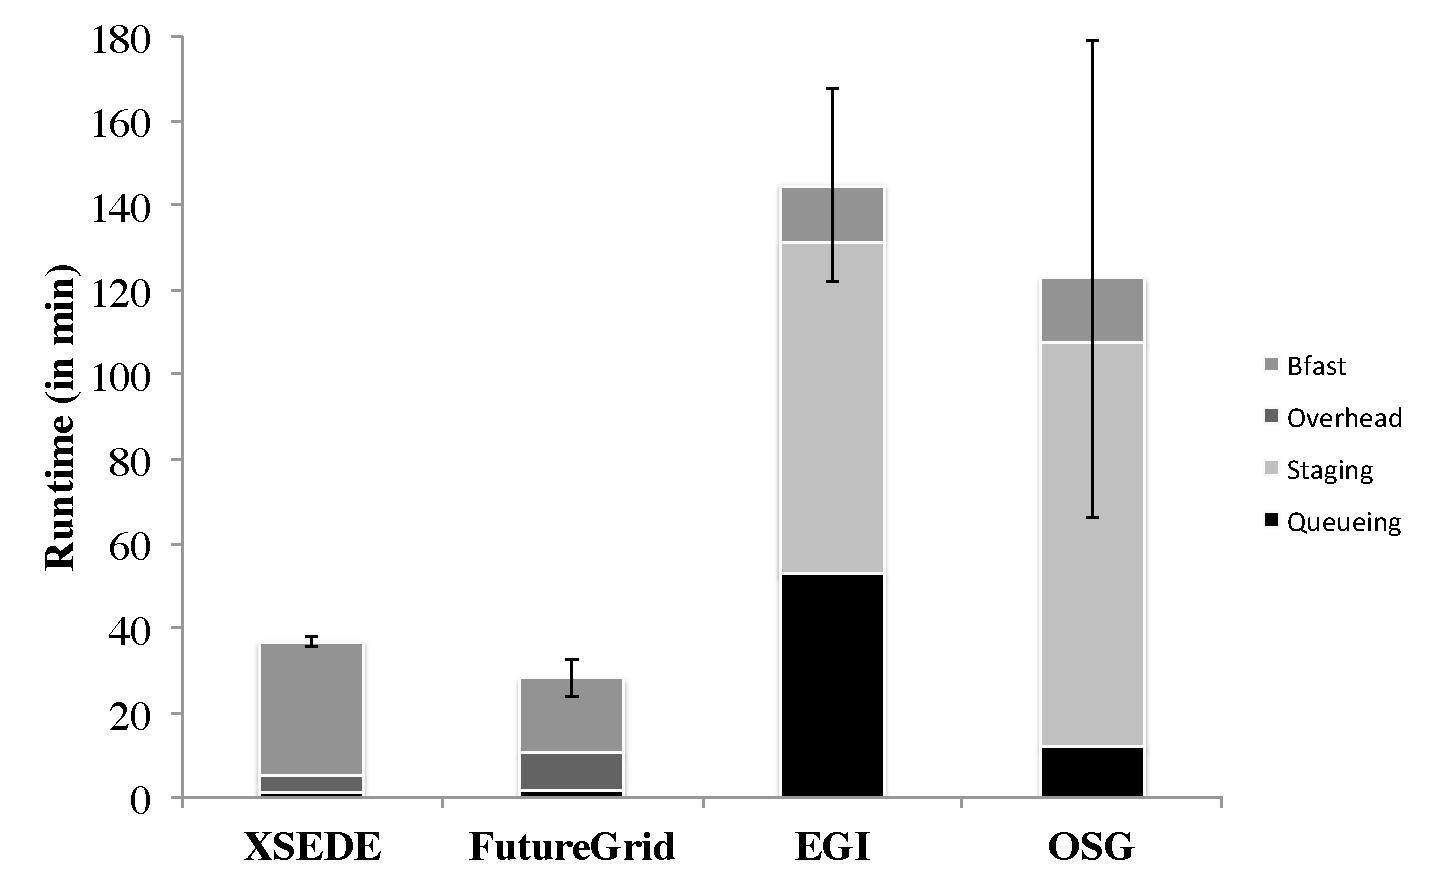
\includegraphics[width=0.45\textwidth]{perf/interop/128-bfast-egi-fg-xsede-osg.pdf}
 \caption{\textbf{PJ Framework Performance on XSEDE, FutureGrid, EGI and 
  OSG:} Running 128 BFAST match tasks on 128 cores. Each experiment is
  repeated at least 3 times. The longer runtimes on EGI and OSG are
  mainly caused by the longer queuing times. Additionally, 
	both infrastructure require the staging of all input files.  \up\up}
	\label{fig:perf_perf-bfast-bj}
\end{figure}

%\jhanote{need to be consistent with case vs scenario}

Figure~\ref{fig:perf_perf-bfast-bj} shows the results of the
experiments. In addition to the runtime we measured the queuing time
(time until \cu state changes to 'Running'), the time to transfer
input files, and the actual runtime of the BFAST \cu. The queue time
include both pilot-external, i.\,e.\ queuing system (PBS, Torque, Condor)
waiting times, as well as pilot-internal waiting times.

% BFAST PERFORMANcE
Generally, the performance of BFAST is heavily dependent on the
available I/O bandwidth. Both the index and read files (7\,GB in this
scenario) need to be loaded into memory. Both Kraken and India use
shared network filesystems (Lustre for Kraken, NFS for India), which
are shared by all jobs running on these machines -- the collective
performance of multiple BFAST \cu thus degrades significantly on
larger machines, such as Kraken, where a potentially large number of
jobs access the filesystem concurrently (the runtime on Kraken is
about 30\,\% slower than on India).  On EGI and OSG, the BFAST \cu
performs best: on OSG about two times faster than on Kraken. This can
mainly be attributed to the use of local disc storage on EGI and OSG
resources.

% Queuing Time
Another interesting factor is the queueing time. In scenario (i) and
(ii), the observed queueing times have been very low, and are mainly
attributed to the BJ internal queue, i.\,e.\ for queuing the sub-jobs
to a BJ agent. In the EGI/DIANE scenario (iii), the queuing time is
dominated by the launch of the 128 worker agents -- each of these
agents needs to be submitted and started via the WMS; on each node, a
DIANE worker agent must be downloaded, installed and started.  In
total, each \cu was required to queue about 50\, min (in comparison to
9\,min for BJ on India/FG).  Thus, even if file staging is not
considered, the scenario executes about 2.3 times slower on EGI
(DIANE) than on FutureGrid (BJ).  The unpredictable queuing time also
contributes to the higher deviation in the measured runtimes. On OSG,
the queuing time is on average 12 minutes, comparable to the queuing
time on XSEDE. 

% File Staging
In the scenarios (i) and (ii), no file staging is used. On EGI and OSG
resources, however, no shared filesystem is available; thus, files
need to be transferred to the executing system. For each \cu, the
reference genome, the index files and one read file need to be staged
(3.38\,GB) -- which consumes more than 50\,\% of the overall runtime.
Thus, the runtime on these two infrastructures is
about 4-5 times longer than on Kraken and India. If file staging is
not considered, OSG shows the best performance of all scenarios
(i)-(iv).
\amnote{The amounts of data differ from what was stated earlier.}
\amnote{The runtime should not be 4 to 5 times longer because of
staging, if staging consumes 50\% of it -- that would give a factor of
2}



% Despite the fact that BigJob has been also installed
% with each run, it shows a significant lower startup time of 73\,sec, i.\,e.\
% about 50\,sec less than DIANE. Additionally, we also observed a runtime
% overhead of about 25\,sec for the DIANE scenario. This overhead is likely
% caused by the additional agents required. While BigJob utilizes one BJ-Agent
% on the resource, DIANE currently requires the spawning of one worker agent per
% \cu that must be executed in parallel. While the Pilot-API marshals these
% differences, i.\,e.\ while the API remains the same for both PJ frameworks, a
% light performance overhead remains observable.


% This
% can mainly be attributed to the better performance of the OSG resource, which is
% particularly visible in the BFAST runtimes, which are on average 40\,\% shorter
% than on LONI. Further, due to the lack of SAGA on OSG, BJ is deployed with the
% Redis c\&c sub-system, which shows a significantly better performance than the
% Advert Service (see section~\ref{sec:pj_performance}).

% \jhanote{What are we trying to say here?  Is it that although the API
%   is similar, semantics of implementation and execution remain
%   different, and that TROY backend handles them?}\alnote{well said}


% This part also sounds too engine-like
% Dynamic
% applications can utilize the elasticity of the TROY resource pool
% e.\,g.\ to improve the time-to-completion and/or to scale the accuracy
% of their computations.

\subsection{Understanding PJ Framework Interoperability\upp\upp}
\label{sec:experiment-interop}

We define two kinds of interoperability: (i) SAGA-based
interoperability, i.\,e.\ the usage of BJ in conjunction with
different SAGA adaptors and infrastructures and (ii) PJ framework
interoperability, i.\,e.\ the usage of different PJ frameworks via the
Pilot-API. For scenario (i) we run BigJob+Pilot-API concurrently on 
FutureGrid::India and XSEDE::Kraken. For scenario (ii) we concurrently run 
BigJob+Pilot-API and DIANE+Pilot-API on FutureGrid::India and EGI as 
well as Condor+Pilot-API and BigJob+Pilot-API on OSG and XSEDE:QueenBee. 
For all scenarios, we run the same BFAST match application described 
in~\ref{sec:fg-xsede-osg-egi} with 64\,\cus on each resource, i.\,e.\ in total 128\,\cus.

\begin{figure}[htbp]
	\centering
	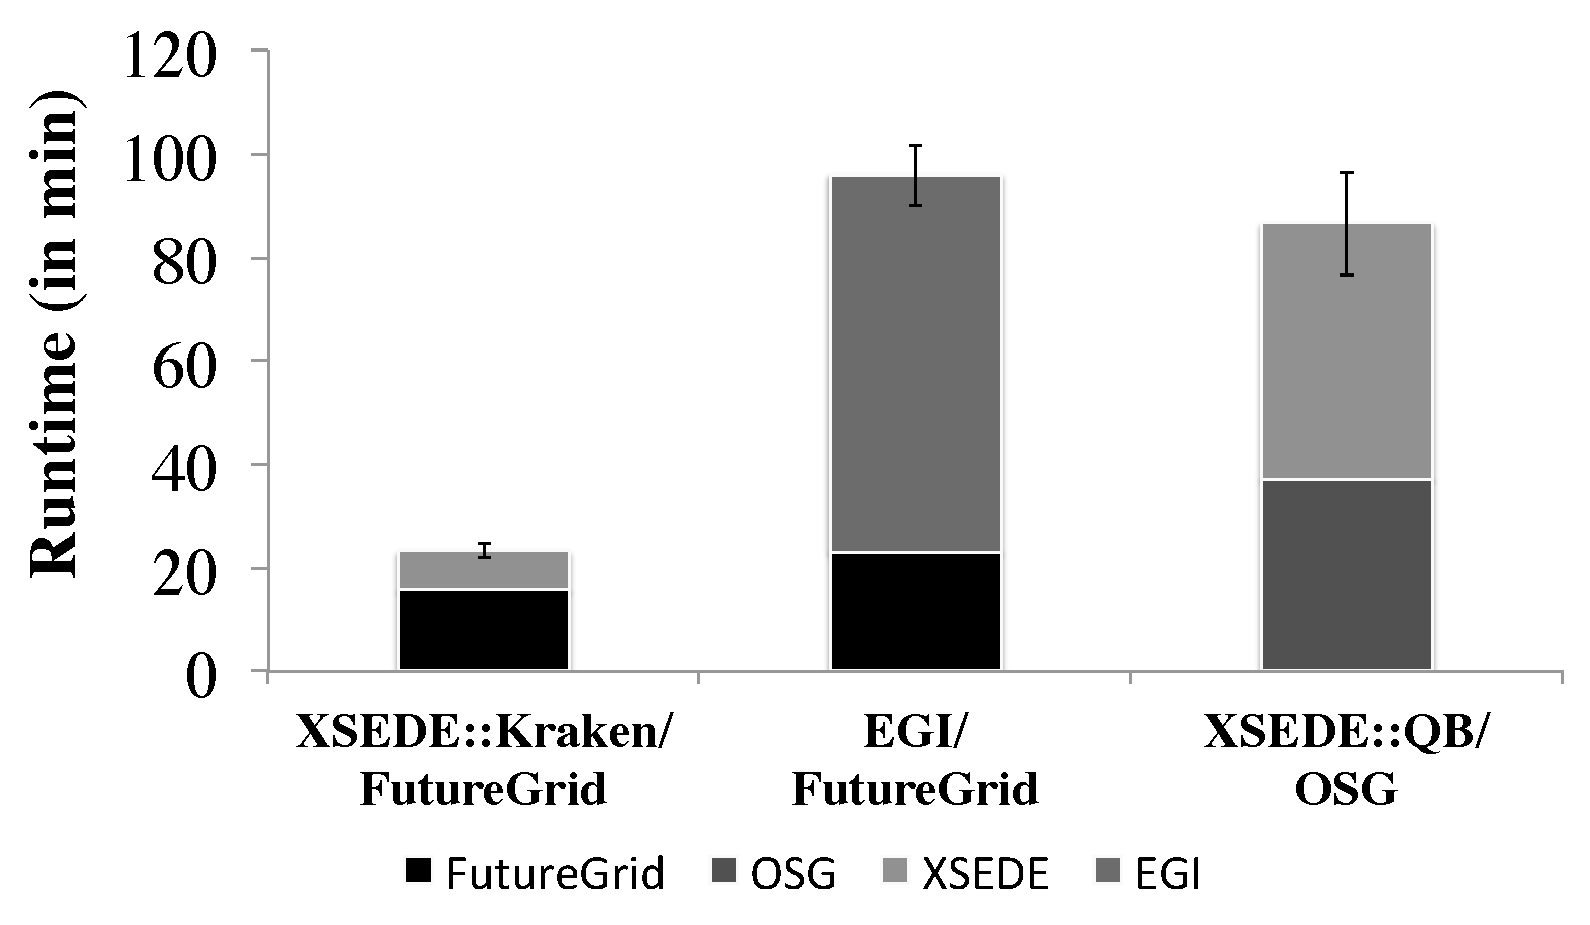
\includegraphics[width=0.45\textwidth]{perf/interop/128-bfast-interop.pdf}
	\caption{\textbf{PJ Framework Interoperability:} Runtime of 128 BFAST \cus 
	on different infrastructures. \cus are equally distributed across the two 
	infrastructures. In particular, slower resources, such as Kraken can benefit 
	from offloading \cus to faster infrastructures.}
	\label{fig:perf_interop_128-bfast-interop}
\end{figure}


Figure~\ref{fig:perf_interop_128-bfast-interop} shows the results of the
interoperability tests. In both scenarios, one \pilot is submitted to each
infrastructure. In scenario (i), one pilot is submitted to Kraken and one to
India. Files are pre-staged before the run. Needless to say, the overall runtime
is determined by the slower resources. Consistent with previous results the
\pilot on India finished before the \pilot on Kraken. The runtime of this
scenario improved about 6\,\% compared to a Kraken only run. This can mainly be
attributed to the usage of the faster India resource. However, the runtime of
the scenario is also about 20\,\% slower than running on India only.

%\jhanote{should this scenario number be different?} \alnote{sorry,
%  just moved this paragraph down from B} 

Finally, scenario (ii) (right bar in
figure~\ref{fig:perf_interop_128-bfast-interop}) demonstrates that two PJ
frameworks can be utilized concurrently using the Pilot-API. Files are
pre-staged for FutureGrid; they need to be staged for the DIANE/EGI \cus. The
performance in this scenario is significantly better than in the DIANE only case
for 128\,\cus (see section~\ref{sec:fg-xsede-osg-egi}), mainly due to the fact
the overhead induced by file staging is only applicable to half of the \cus.
However, it must also be noted that the performance of the BJ \pilot is about
30\,\% worse for the EGI/FG run compared to the XSEDE/FG run. This can be mainly
attributed to the distributed coordination necessary in a high latency
environment. All communication is conducted via a Redis instance deployed on FG.
In scenario (ii) the BJ manager is deployed on EGI; thus, for each \cu several
cross-atlantic roundtrips are necessary.

In summary, the Pilot-API enables applications to utilize a dynamic
resource pool consisting of resources of different infrastructures, e.\,g.\ EGI
and FutureGrid, but also XSEDE resources, at large-scales hitherto unattainable.



\section{P* as a Model for Pilot-Data\upp\upp}
\label{sec:pilot-data}
% \alnote{remove emphasis on dynamic execution} \jhanote{Motivation for
%   P* model for data: (i) Distributed data placement not done
%   effectively or scalably; (ii) unable to handle dynamic
%   (late-binding) issues or multi-stage dependencies, (iii) further
%   optimizations}\alnote{see first version below}

Many scientific applications have immense data requirements, which are
projected to increase dramatically in the near
future~\cite{hey2009}. The small genome alignment tool
scenario presented above e.\,g.\ operates on a input data set of
$>7$\,GB. While Pilot-Jobs efficiently support late-binding of
\computeunits and resources, the management of data in distributed
systems remains a challenge due to various reasons: (i) the placement
of data is often decoupled from the placement of Compute Units and
Pilots, i.\,e.\ the application must often manually stage in and out
its data using simple scripts.  (ii) heterogeneity, e.\,g.\ with
respect to storage, filesystem types and paths, often prohibits or at
least complicates late binding decisions. (iii) higher-level
abstraction that allow applications to specify their data dependencies
on an abstract, logical level (rather than on file basis) are not
available. (iv) due to lack of a common treatment for compute and
data, optimizations of data/compute placements are often not
possible. For example, in scenario (iii) and (iv) presented in
section~\ref{sec:fg-xsede-osg-egi}, even though the 50\,\% of the
input data set is shared for all \cus, the complete data is staged for
each \cu.

In addition, applications must cope with various other challenging,
data-related issues, e.\,g.\ varying data sources (such as sensors
and/or other application components), fluctuating data rates, transfer
failures, optimizations for different queries, data-/compute
co-location etc. While these issues can be in principal handled in an
application-specific way, the usage of higher-level abstractions, such
as a common \pilot-based abstraction for compute and data is
preferable.  

% Thus, having defined the P* model, we explore its extension to data.

This motivates an analogous abstraction that we call \emph{\pilotdata
  (PD)}. \jwave{PD provides late-binding capabilities for data by
  separating the allocation of physical storage and application-level
  data units.} Further, it provides an abstraction for expressing and
managing relationships between data units and/or work units. These
relationships are referred to as \emph{affinities}.

% \jhanote{difficult to use affinity without defining it..}
% \alnote{tried to describe affinities a little bit better}

%\alnote{Extension vs. Application vs. Translation}
\subsubsection*{P* Model Elements for Data}

% A Pilot-Data Framework facilitates the late-binding between data units
% and physical storage resources, the so called pilot-stores.

The elements defined by P* (in section~\ref{sec:p_star_elements}) can
be extended by the following elements:

%\alnote{What is the role of SU in Data?}
\begin{compactenum}[A.]

\item \textbf{\pilot (Pilot-Data):} A \pilotdata (\pd) functions as a 
	placeholder object that reserves the space
	for data units. PD facilitates the late-binding of data and resource and is
	equivalent to the \pilot in the compute model.

\item \textbf{Data Unit (DU):} DU is the base unit of data assigned by
  the application,  e.\,g.\ a data file or chunk. Multiple DUs can be aggregated 
   within a Data Unit Set.

% \item \textbf{Pilot-Data (PD):} PD allows the logical grouping of DUs
%   and the expression of data-data affinities. This collection of files
%   can be associated with an extensible set of properties. One of these
%   properties is affinity. 

\item \textbf{Scheduling Unit (SU):} is an internal unit of scheduling (as in 
the compute case). The Pilot framework can aggregate or split DUs into one 
or more SUs.

\item The \textbf{Pilot-Manager (PM)} is the same as in the compute model and
implements the different characteristics of the P* model. It is responsible for
managing \dus and \sus. Data is submitted to the framework via the PM. The PM
which is responsible for mapping \dus to \sus and for conducting decision 
regarding resource assignments. \sus are placed on physical resources via the \pilot.
	
\end{compactenum}
 
Note, each element can be mapped to an element in the P* Model by
symmetry, e.\,g., a DU correspond to a \cu  in the original P* Model; 
a PD is a placeholder reserving a certain amount of storage on a physical 
resource and corresponds to the \pilot in the P* Model.

% \jhanote{PJ Model is confusing. Either it is P Model or PJ
%   Framework} \alnote{ok}

% A particular critical requirement for data-intensive application, is
% the management of affinity between DUs and also between \cus and
% DUs. Thus, Pilot-Data introduces the PD container object for
% expressing relationships between DUs. A PD corresponds to an SU in
% the \jwave{PJ model}, i.\,e.\ it is used as scheduling unit for
% internal optimizations, e.\,g.\ the grouping of DUs. Having
% instantiated a PD, it can be assigned to a PS via the PD manager. A
% PS is a placeholder reserving a certain amount of storage, i.\,e.\
% it corresponds to a pilot in the pilot-job model. By associating a
% PD to a PS the data is actually moved to the physical location
% associated with the PS. The PD manager facilitates the creation of
% PSs, schedules data movements (with respect to specified affinities)
% and manages data accesses.

\subsubsection*{P* Model Characteristics for Data}

While the extended P* Model introduces new elements, the
characteristics however, remain the same to a great extent. The
coordination characteristic describes how the elements of PD interact,
e.\,g.\ utilizing the M/W model; the communication characteristic can
be applied similarly. The scheduling characteristics must be extended
to not only meet compute requirements, but also to support common data
access patterns. \jhanote{Propose comment out due to space
  restrictions: The scheduling component particularly needs to
  consider affinities, i.\,e.\ user-defined relationships between \cus
  and/or \dus. Data-data affinities e.\,g.\ exist if different \dus
  must be present at the same compute element; data-compute affinities
  arise if data and compute must be co-located for a computation, but
  their current location is different.} Data and compute placement
decisions are made by the scheduler based on defined policies,
affinities \& dynamic resource information.


\subsubsection*{Pilot-API for Data} 
Analogous to the Pilot API for Compute, the Pilot Data API~\cite{pilot_api} 
defines the \texttt{PilotDataService} entity as an abstraction for creating and
managing pools of storage. A \texttt{PilotData} instance represents the actual
physical storage space. The \texttt{ComputeDataService} entity
functions as an application-level scheduler, which accepts both
\texttt{ComputeUnits} and \texttt{DataUnits}. It resolves necessary
dependencies (e.g. data/data or data/computer affinities), and is
responsible for managing the execution of \dus and \cus.



% \subsubsection*{BigData: A SAGA-based Pilot-Data Prototype for TROY}
\label{sec:bigdata}

\begin{figure}[t]
    \centering
    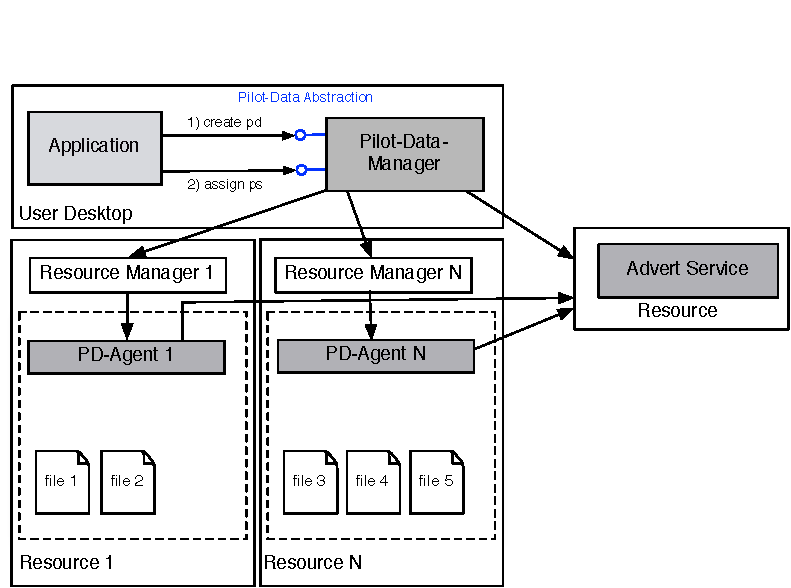
\includegraphics[width=0.48\textwidth]{figures/pilot-data-manager.pdf}
    \caption{\textbf{BigData Architecture:} The BD Manager exposes
      TROY's PD API. Application can create group of files and assign
      files to storage. The BD manager tracks file locations in the
      data catalog. The scheduler optimizes data-compute co-location.
      The transfer manager initiates and monitors data
      movements. \up\up}
    \label{fig:pilot-data-architecture}
\end{figure}

% \begin{figure*}[t]
%   \up\up\up
%   \begin{minipage}[t]{0.475\linewidth}
%     \centering
%     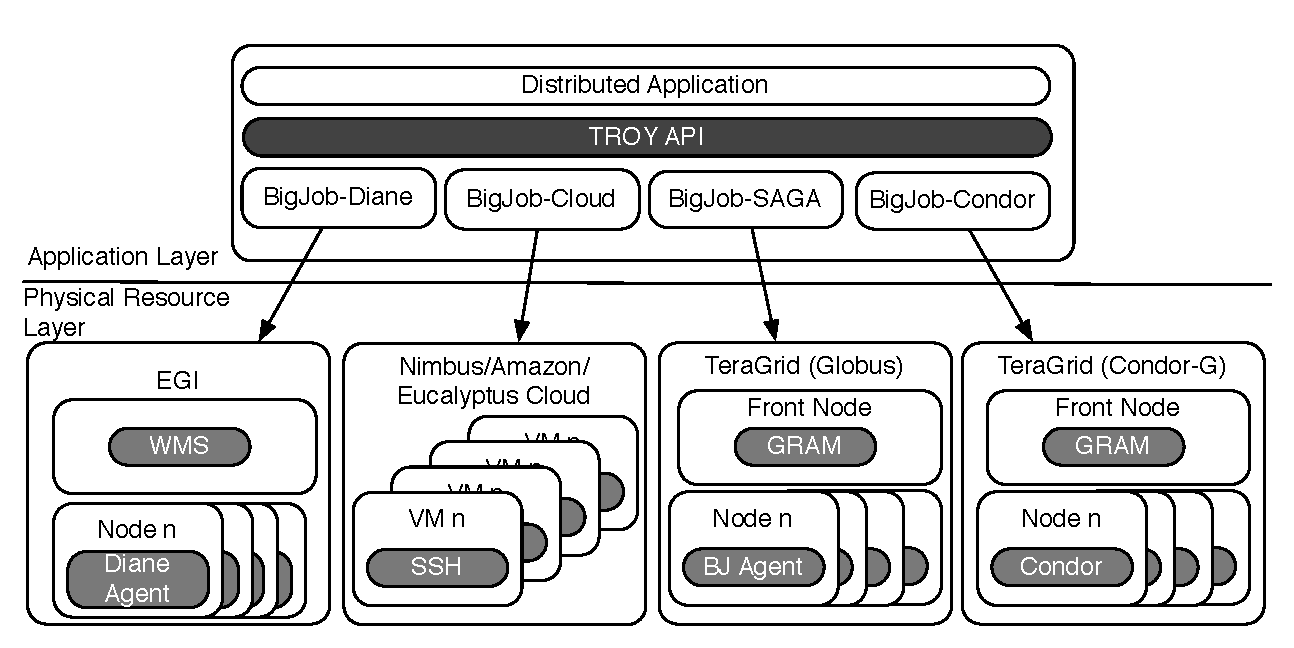
\includegraphics[width=\textwidth]{figures/distributed_pilot_job.pdf}
%     %\includegraphics[width=\textwidth]{figures/P1140340.JPG}
%     \caption{\textbf{BigJob -- SAGA-based Pilot-Job Implementation:}
%       BigJob is the implementation of the actual PJ functionality for
%       TROY. SAGA BigJob permits usage with multiple middleware
%       backends~\cite{}}
%     \label{fig:figures_distributed_pilot_job}
%     \end{minipage}
%   \hspace{0.035\linewidth}
%   \begin{minipage}[t]{0.475\linewidth}
%     \centering
%     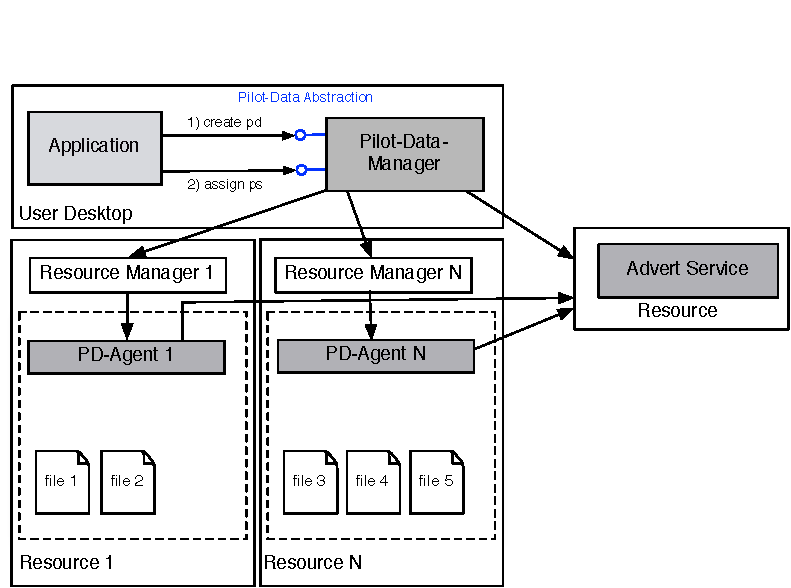
\includegraphics[width=\textwidth]{figures/pilot-data-manager.pdf}
%     \caption{\textbf{BigData Architecture:} The BD Manager exposes
%       TROY's PD API. Application can create group of files and assign 
%       files to storage. The BD manager tracks file locations in
%       the data catalog. The scheduler optimizes data-compute co-location.
%       The transfer manager initiates and monitors data movements. \up\up}
%     \label{fig:pilot-data-architecture}
%     \end{minipage}
% \end{figure*}

BigData-SAGA is the SAGA-based prototype of the Pilot-Data
abstraction; in the scope of this paper it is referred to as simply
BigData (BD).  Figure~\ref{fig:pilot-data-architecture} gives an
overview of the architecture.  The system consists of two components:
the BD manager, and the BD agents deployed on the physical
resources. The coordination scheme used is again M/W with some
intelligence that is located de-centrally at the BD agent. As
communication mechanism the SAGA Advert Service is used, in a similar
push/pull mode as for BJ.

The BD manager is responsible for 1) meta-data management, i.\,e.\ it
keeps track of the pilot stores that a pilot data object is associated
with, 2) for scheduling data movements and data replications (taking
into account the application requirements defined via affinities), and
3) for managing data movements activities.  Similar to BigJob, an
agent on each resource is used to manage the physical storage on a
resource.  

A particular critical requirement for data-intensive application, is
the management of affinity between DUs and also between WUs and
DUs. The BD scheduler supports preliminary affinity-aware
scheduling: both BigJob and BigData are tightly integrated to
efficiently support compute- and data-related aspects of dynamic
execution (see also \S{IIIA}).
 
\jhanote{Andre, please review the next paragraph: Should it just go
  for simplicity?} Thus, Pilot-Data introduces the PD container object
for expressing relationships between DUs. A PD corresponds to an SU in
the P* Model, i.\,e.\ it is used as scheduling unit for internal
optimizations, e.\,g.\ the grouping of DUs. Having instantiated a PD,
it can be assigned to a PS via the PD manager. A PS is a placeholder
reserving a certain amount of storage, i.\,e.\ it corresponds to a
pilot in the pilot-job model. By associating a PD to a PS the data is
actually moved to the physical location associated with the PS. The PD
manager facilitates the creation of PSs, schedules data movements
(with respect to specified affinities) and manages data accesses.


%%%%%%%%%%%%%%%%%%%%%%%%%%%%%%%%%%%%%%%%%%%%%%%%%%%%%%%%%%%%%%%%%%%%%%


% In addition to the three Pilot-Job framework discussed in this section, various
% other frameworks exist.
% \begin{itemize}
%     \item MyCluster~\cite{1652061} enables the 
% creation of a Condor, PBS or SGE clusters on-demand.
%     \item Falkon~\cite{1362680} is a Pilot-Job framework that emphasizes the 
% performance of its task dispatcher.
%     \item Nimrod/G~\cite{10.1109/HPC.2000.846563}
%     \item DIRAC~\cite{1742-6596-219-6-062049} is another pilot-job framework 
% used by the LHCb community.
%     \item ToPoS~\cite{topos} is a REST-based web service primarily designed with 
% respect to parameter sweep applications. Internally, ToPoS utilizes PJ 
% capabilities to efficiently manage resources.
%     \item The Production and Distributed Analysis System 
% (PanDA)~\cite{1742-6596-219-6-062041} is the workload management system of 
% the ATLAS experiment. PanDA utilizes multi-user PJs for resource management. 
% The PJ component is built on top of Condor-G and referred to as AutoPilot. 
% It can also be used independently of the ATLAS environment. 
% \end{itemize}


% 
% Both BigJob and BigData define similar elements that can be mapped to
% each other. Nevertheless, compute and data model sometimes require a
% different treatment.  The extended TROY (an implementation of the
% extended P* Model) will optimize data- and computing according to a
% set of defined affinities and policies.

% BJ and BD encapsulate cross-cutting properties across data and
% computation. 

% With the maturing of both models and
% implementations, we expect that both the PJ and PD model converge in
% the future.

\section{Discussion and Future Work \upp\upp}
\label{sec:discussion-future-work}

% The P* model was used to demonstrate
% We established PJ and PD as abstractions for supporting dynamic
% execution by decoupling workload and resource
% assignment/scheduling. 

% they share different important properties with respect to the commonly
% used communication and coordination schemes.

% \alnote{Add discussion on limitations of API - address these
%   limitations in a common runtime system.}

The primary intellectual contribution of this work has been the
development of the P* Model, the mapping of P* elements to PJ
frameworks such as DIANE and Condor-G/Glide-in, its validation via the
Pilot-API and demonstration of its use with multiple PJ frameworks.
 
The P* Model provides a common abstract model for describing and
characterizing Pilot-abstractions. We validate the P* Model by
demonstrating that the most widely used PJ frameworks, viz., DIANE and
Condor-G/Glide-in can be compared, contrasted and analyzed using this
analytical framework.

The Pilot-API captures the commonalities between the different PJ
frameworks and provides a common access layer to them via a uniform
API; it also enables the concurrent use of multiple PJ frameworks,
thus providing interoperability and extensibility.

% , i.\,e.\ the architecture and the communication and coordination
% schemes.\alnote{i.e. sub-clause can go} .  Building on the P* Model,
% the Pilot-API's design enables the easy exchange of PJ
% implementations, and also The Pilot-API functions as common access
% layer for different PJ frameworks, thus


% However, the SAGA inspired approach to the Pilot-API design and the
% leverage of the design and deployment experiences of SAGA, e.\,g.\ by
% moving the responsibility of correctly deployed grid-middleware to the
% resource providers and not the end-users, should be an effective
% solution. 

P* provides significant future development, research \& deployment
opportunities. We discuss one opportunity along each of these axes:
(i) Development and Extension: In order to overcome limitations of the
API-based approach we will develop a complete implementation of the P* Model
-- called TROY (Tiered Resource Overlay). TROY will provide deeper
integration of the Pilot-API via a semantic mapping of the P* elements
and characteristics to \pilotjob frameworks.  TROY will also provide a
unified -- compute and data, implementation of P*, e.g., BigData
analogous to BigJob.  (ii) Research Issues: These developments and
extensions will also provide the basis to explore and reason on the
relative roles of system versus application-level scheduling,
heuristics for dynamic execution and the role of affinity; (iii)
Deployment and Uptake: The Pilot-API and TROY are/will be designed to
support production scale science on production infrastructure (as
demonstrated by the emphasis on production infrastructure in our
experimentation).  Our experience with fragile grid middleware and
infrastructures has taught us to appreciate the significance of the
ease of deployment and the need for robustness of tools and software
on heterogeneous distributed infrastructures.  TROY -- which embodies
the P* Model, is being designed with usability, reliability and
robustness as first-class considerations.

Our fundamental research has immense practical implications and
potential: Although current PJ frameworks collectively support
millions of tasks yearly on several production distributed
infrastructure, extensibility and interoperability remain significant
challenges~\cite{extenci}.  Given the increasing importance of
pilot-jobs and the challenges associated with distributed data
placement, our work which provides both a conceptual model and
practical solutions has the potential to improve this situation.
In fact, it is a stated goal of our research to enhance the range of
applications and application usage-modes that will benefit from the
pilot abstraction, by deeply integrating P* and TROY capabilities with
multiple production infrastructures.





% On the basis of successful validation of the P* Model, we propose
% extensions to include data.  For example, presenting unified
% abstractions within the Pilot-API and

% Additionally we aim to provide explicit support for advanced dynamic
% execution modes and 

% In summary, we will use existing and emerging capabilities of TROY to
% support the efficient and scalable solution of many scientific
% applications that involve multiple independent tasks.\alnote{just one sentence - can be merged with paragraph above.}

% It is not possible to anticipate all of the tools and abstractions
% that distributed applications will need down the road. Changes in
% infrastructure and application requirements cannot be predicted. For
% this reason, tools must provide open interfaces to enable more easy
% integration and interoperation with other tools. Whether this can be
% best achieved by new extensible tools or “tool orchestration” or a
% tool “framework” is an open question. This, of course, does not
% preclude the internal evolution of existing tools to implement new
% abstractions, but just this is not enough in our view.

\up
\section*{Acknowledgements\upp\upp}
\footnotesize{This work is funded by NSF CHE-1125332 (Cyber-enabled
  Discovery and Innovation), HPCOPS NSF-OCI 0710874 award, NSF-ExTENCI
  (OCI-1007115) and NIH Grant Number P20RR016456 from the NIH National
  Center For Research Resources. Important funding for SAGA has been
  provided by the UK EPSRC grant number GR/D0766171/1 (via OMII-UK)
  and the Cybertools project (http://cybertools .loni.org; PI Jha)
  NSF/LEQSF (2007-10)-CyberRII-01. SJ acknowledges the e-Science
  Institute, Edinburgh for supporting the research
  theme. ``Distributed Programming Abstractions'' \& 3DPAS. MS is
  sponsored by the program of BiG Grid, the Dutch e-Science Grid,
  which is financially supported by the Netherlands Organisation for
  Scientific Research, NWO. SJ acknowledges useful related discussions
  with Jon Weissman (Minnesota) and Dan Katz (Chicago). We thank J Kim
  (CCT) for assistance with BFAST.  This work has also been
  made possible thanks to computer resources provided by TeraGrid TRAC
  award TG-MCB090174 (Jha) and BiG Grid.  This document was developed with
  support from the National Science Foundation (NSF) under Grant No. 0910812
  to Indiana University for ``FutureGrid: An Experimental, High-Performance
  Grid Test-bed''.}  \up
%\bibliographystyle{plain}
\bibliographystyle{IEEEtran}
\bibliography{pilotjob,saga,saga-related}
\end{document}


\note{Facilities provided include the creation of a PJ, insertion of
  tasks, and attachment to a CPU resource pool for late-binding task
  execution.}  \note{Tasks are ultimately loaded onto specific
  resources using the pilot-job and late-binding. In other words}
\note{PJ provides a mechanism to decouple “task coordination” from
  “resource mapping”.}




% To perform the above experiments we built an application \smnote{this
% application is DARE. do we need mention it here?} using TROY API to submit Bfast
% \cu 's with different input files to different backend implementations. The \cu 's
% are completely handled and submitted to different backends by TROY and the
% co-ordination of \cu 's was made simple for the application. Further, applications
% can also continuously monitor status of remote agents and UOWs.

% Further, it shows that both PJ implementations can be used
% concurrently. This is particularly useful if the time-to-completion can be
% reduced in cases where resources on another infrastructure are available.





% Figure~\ref{fig:perf_perf-bfast-bj} shows the results of the
% experiments. The time-to-completion for TROY-DIANE is about 207\,sec
% longer than for TROY-SAGA. The main contributor for this increased
% runtime is the deployment time required for DIANE. In a multi-node
% setup multiple work agents must be used (8 in this case).  For each
% worker agent DIANE must be downloaded, installed and started
% separately. In total this requires about 178\,sec. Further, each DIANE
% worker agent is queued as a separate job at the local resource manager
% -- this contributes the the higher deviation in the measured
% runtimes. Because BigJob requires a pre-run installation on each site,
% it only shows a startup time of 28\,sec. Additionally, we also
% observed a runtime overhead of about 17\,sec for the TROY-DIANE
% scenario. This overhead is likely caused by the additional agents
% required.

% % In the case of BJ-DIANE backend Multinode submitter was not used/not % yet. As
% a result it submits job request's for each node separately and there % also some
% delay between actual launch and startup time of UOW. Further, DIANE % was
% installed separately for every agent/node requested.

% \alnote{commented out for submission: A reflection on the Reality of Distributed Infrastructures}

%\subsection{A reflection on the Reality of Distributed Infrastructures}



% Further, TROY hides many of the complications with various pilot
% jobs like multiple node backend agents, how \cu 's distribution to
% various backends. Thus, this enables users of this API to
% concentrate more on designing their applications instead worrying
% about the various configurations of the pilot jobs.

However, even for traditional
high-performance/parallel applications, the evolution or internal
dynamics of an application may vary, thereby changing the resource
requirements.  For example, different solvers, adaptive algorithms
and/or implementations, can also require applications to utilize
different set/amounts of resources.  Thus, the need to support dynamic
execution is widespread for computational science applications.

% PJ provide a simple model for distributed resource usage.
% Pilot-jobs enable this decoupling typically in user-space without the
% policy-level complexity of implementing advanced reservations. 

%Pilot-jobs typically in user-space (i.e. application-level
%scheduling).  

%Although there are many implementations of the PJ abstraction

% , and are, in general, expensive to develop and manage in terms of
% the time and effort involved.  T Tools tend to be customized to
% specific applications and their requirements, with limited concern
% for reuse or extensibility. For example de- spite community efforts
% such as CCA, few applications, if any, mix-and-match components
% developed by different projects.

% In fact, not only do distributed applications need abstractions to
% support the requirements through the individual stages of
% development, deployment and execution, support for applications
% through these stages needs to be a coherent integrated activity, as
% opposed to a disjointed effort..  There are just too many moving
% parts!
% pilot-data % (PD) 

% to treat data as a first-class schedulable entity, is a concept
% analogous to PJ:

%  We present and discuss
% the P* model in \S{II}.


% Both PJ/PD frameworks rely on SAGA for implementation
% of the actual PJ/PD functionality. 
% Using the adaptor mechanism, TROY
% can further be extended to other PJ implementations.

% \jhanote{Note the distinction between pilot-jobs and pilot-job
%   framework: DIANE, Swift are PJ frameworks. Specific instances of
%   these tools/usage give rise to pilot-jobs.}\alnote{added PJ
%   framework definition to terms and usage.}

% which exposes
% the semantics of PJs in a P* conform way, and a runtime
% environment. 
% \alnote{OLD: As we will discuss, consistent with the goals and aims of
%   SAGA, there can be multiple instances of BigJob for different
%   backends.}\jhanote{Have we not gone to multiple instances of the
%   Pilot-Job for TROY and not multiple instances of
%   BigJob?}\alnote{refined}
% and outline briefly how other well known pilot-jobs can be
% understood using the {\it vectors}~\cite{dpa_surveypaper} of the P*
% Model.
% \alnote{do we validate just the TROY API or the TROY framework?}



% \jhanote{Should we to introduce Dynamic Applications explicitly in the
%   title? Just a question, not a suggestion...}

%\subsection{Introduction \jhanote{SJ, AL}}


%\section{Pilot-* : An abstraction for Dynamic Execution}
%\section{TROY: A Model of Pilot-Abstractions for Dynamic Execution}



% Figure~\ref{fig:figures_pstar}
% illustrates the interactions between the elements of the P*
% model. Although there can be variations, a typical usage scenario
% consists of the following steps: The application specifies the
% capabilities of the resources required (step 1).  \jhanote{Andre,
%   Mark: Is Step 1 true? Couldn't we just say: application specifies
%   the \cu ?} During the instantiation of a PJ and the assignment of
% resources to the PJ, pilots are queued and started via the local
% resource manager (step 1-4).
% 
% \jhanote{We should talk about ``API'' --- \cu  crossing P* API, ie
%   controlled by Pilot-Manager, and then becoming an SU thereafter.
%   Also talk about multi-level scheduling. Anything that focusses the
%   reader's attention on an understanding that was not covered in brief
%   description} \alnote{refined}
% 
% Commonly, the pilot-manager (PM) can be accessed via a set of command
% line tools and/or an API via which an application can create and
% submit \cus to the pilot-manager (step 5/6). A \cu  that is submitted
% becomes a SU, i.\,e.\ the PM is now in control of it and schedules and
% manages its execution. In the simplest case one \cu  corresponds to one
% SU; however, SUs can be combined and aggregated to optimize
% throughputs and response times.
% 
% Commonly, a hierarchical M/W coordination model is used: On
% the first level, the PM uses M/W in order to coordinate the actions of
% the pilots that are part of its resource pool (usually 1 or
% more). Once a SU is forwarded to a pilot, the pilot is responsible for
% the coordination of the SU execution. Again a pilot usually manages 1
% or more SUs using M/W. \jhanote{Need some clarification: what is the
%   worker/agent here? (i) Isn't it PJ Frameworks that use M-W
%   coordination and not the PJ.  Also, in the framework, isn't the
%   Manager the Master, and the Pilot-Job the Worker; What about \cu /SU ?
%   ie if \cu /SU are the workers, what is the master?}  \alnote{refined}
% Scheduling decisions can be conducted on each level. The delegation of
% decision capabilities into lower levels, i.\,e.\ the pilot, can yield
% to a more autonomic and adaptive behavior as well as a better
% scalability.
% 
% \alnote{TODO: remove redundancy with paragraph above} As explained, a
% P* implementation usually operates a hierarchy of schedulers.  The
% following examples involves a two-level hierarchy: In the first
% hierarchy level the PM schedules an SU to a pilot of its resource pool
% (step 7). Another round of scheduling can occur within the pilot,
% i.\,e.\ the pilot decides when and on what physical resource a SU is
% executed (step 8). Further, the pilot manages the subsequent execution
% of the SU on the physical resource on which the pilot is operating.



% \jhanote{Integrate.. next sentence} PJ frameworks with decentralized
% decision often utilize autonomic agents that accepts respectively pull
% SUs according to a set of defined policies.


% \alnote{We use the term agent to denote a component inside the pilot
%   that has some decision making capability. In most cases we could
%   replace agent just with pilot. However, when talking about decentral
%   coordination with autonomic decision making this will be
%   difficult. Should we explicitly define an agent in sec II under
%   Pilot-Job (aka pilot)?}
 


%or the implementation of a custom scheduler is supported.
% \jhanote{Move to an appropriate location}\jwave{Commonly }
% \jhanote{Mention that application/user level input/heuristics can be
%   employed at either of the two stages: binding and/or scheduling}
% \jhanote{Candidate for removal}\jwave{Furthermore, the time of binding
%   influences the point at which the binding decision is made, e.\,g.\
%   in the case of early binding, the decision could be made by the
%   application, while in late binding mode the decision is made by the
%   PJ framework.}
% \jhanote{Integrate: Note that that this can either be a simple
%   grouping or a smart aggregation of \cus (e.\,g.\ two sets of
%   parameters merged into one).}

% \note{TROY provides a unified API that can be used to expose various
%   PJ frameworks (e.\,g.\ BigJob, DIANE and Condor-G). Further, it
%   enables the concurrent usage of multiple PJ frameworks (see
%   figure~\ref{fig:figures_distributed_pilot_job}).  The SAGA inspired
%   approach to TROY's API design --- its SAGA inspired adaptor-based
%   architecture, leverage the design experiences of SAGA, are appealing
%   to the pilot-job user community. Also, the chosen designs enables
%   the easy exchange of PJ implementations and the concurrent use of
%   multiple PJ frameworks. TROY thus functions as common access layer
%   for different PJ frameworks, providing interoperability and
%   portability of PJ applications. To some extent, the TROY API can be
%   considered to be a prototype of a PJ-like API extension to SAGA (see
%   Discussion \& future work, \S\ref{sec:discussion-future-work}).}
